\appendix

\section*{Appendix}
The appendix includes the following sections:
\begin{itemize}
\itemsep0em
    \item \S\ref{supp:model} - Model Details
    \item \S\ref{supp:training} - Training Details
    \item \S\ref{supp:eval} - Evaluation Details
    \item \S\ref{supp:data} - Datasets Details
    % \item \S\ref{supp:dataexamples} - Dataset Examples
    \item \S\ref{supp:limit} - Limitations and Potential Solutions

    % \item \S\ref{supp:related_work} - Related Work
\end{itemize}

\section{Model Details}
\label{supp:model}

This appendix expands the model description in Sec.~\ref{sec:pretraining} and
Sec.~\ref{sec:posttraining}. \molmoactt is built in two architectural stages.
First, \molmoacttpre adapts the \molmoer vision-language backbone into a
discrete autoregressive robot policy. It keeps the Molmo2 visual and text token
interface, but adds robot-specific state, setup/control, and action-output
tokens so that robot trajectories can be trained with the same next-token
objective as vision-language data. Second, post-training attaches a continuous
DiT-style action expert to this already robot-aware backbone. The expert uses
per-layer KV conditioning on the VLM and learns a flow-matching velocity field
over continuous robot action chunks. \molmothink keeps the same architecture and
adds an autoregressive depth-token prefix before action prediction.

\subsection{\molmoactt Backbone}
\label{supp:model-backbone}

\paragraph{Backbone initialization and visual inputs.}
\molmoactt initializes from \molmoer, a Molmo2-based VLM specialized for
embodied and spatial reasoning. The backbone therefore follows the Molmo2
architecture~\citep{clark2026molmo2openweightsdata}: visual inputs are encoded
by a SigLIP2 vision transformer, pooled and projected by a vision-language
connector, and consumed by an autoregressive language model together with text.
The important MolmoAct2-specific choice is how this interface is used for robot
control. Robot examples can include multiple camera views, proprioceptive state
tokens, setup/control descriptors, and action targets, so sequence length is a
central constraint. For the robot-policy stages in Sec.~\ref{sec:pretraining}
and Sec.~\ref{sec:posttraining}, each camera observation is represented as a
single resized crop rather than a tiled high-resolution image. Video examples
are sampled at up to 2 FPS and capped to at most 8 frames. Multi-camera robot
episodes are serialized as multiple image inputs, and the camera order is
randomized at the episode level during pre-training.

\paragraph{Vision encoder and connector.}
Each crop is encoded by a SigLIP2 vision transformer~\citep{tschannen2025siglip}.
The connector follows the Molmo2 design. It reads patch features from the
third-to-last and ninth-from-last ViT layers, then pools local windows with a
multi-head attention layer. For images, \(2\times2\) patch windows are pooled
into one visual token using the mean patch feature as the query. For videos, a
\(3\times3\) pooling window is used to further reduce the number of frame
tokens. The pooled features are projected into the language-model embedding
space with a shared MLP. This produces a sequence of visual tokens that can be
interleaved with text tokens.

\paragraph{Language model input.}
The language model receives visual tokens together with the robot instruction
and robot-specific text. Multi-camera observations are identified by image-index
text, and video frames use the same frame markers as Molmo2. Since MolmoAct2
robot observations use single resized crops, the model does not rely on the
multi-crop column-token machinery for robot control. Visual tokens are allowed
to forward-attend to one another, including across different frames or camera
views, so the backbone can reason over the full visual context before producing
state-conditioned robot outputs.

\paragraph{Added tokens.}
The robot interface keeps the model in the same autoregressive format as the
base VLM by adding robot-specific tokens to the backbone vocabulary. A robot
example contains visual observations, a language instruction, optional setup
and control descriptors, discrete state tokens, and an output marker that tells
the model which response type to produce. The main markers are
\texttt{\detokenize{<setup_start>}}, \texttt{\detokenize{<setup_end>}},
\texttt{\detokenize{<control_start>}}, \texttt{\detokenize{<control_end>}},
\texttt{\detokenize{<state_start>}}, \texttt{\detokenize{<state_end>}}, and
\texttt{\detokenize{<action_output>}}. We also add indexed token families for
discrete robot quantities: action tokens
\texttt{\detokenize{<action_0>}}--\texttt{\detokenize{<action_2047>}} and
state tokens
\texttt{\detokenize{<state_0>}}--\texttt{\detokenize{<state_255>}}. The
depth tokens are added only for \molmothink post-training: the model uses
\texttt{\detokenize{<depth_output>}}, \texttt{\detokenize{<depth_start>}}, and
\texttt{\detokenize{<depth_end>}}, together with depth-code tokens
\texttt{\detokenize{<depth_0>}}--\texttt{\detokenize{<depth_127>}}.

Setup and control descriptors make embodiment and action semantics explicit in
the prompt. For example, a bimanual YAM prompt can indicate that the robot is a
pair of YAM arms and that the control target is an absolute joint pose, while a
DROID prompt can indicate a Franka arm with delta end-effector control. This
lets the same tokenizer and backbone support different robots without forcing
all datasets into a single physical coordinate convention.

Continuous robot states are normalized using dataset statistics and discretized
into one of 256 state tokens per scalar dimension. The resulting state-token
sequence is appended to the prompt before the action output marker. Continuous
actions are normalized, padded to a maximum width of 32 dimensions, and encoded
by \molmoactfast into discrete action tokens with a 2048-token action
vocabulary. During pre-training, these action tokens are the only robot target.
During post-training and fine-tuning, the same example also provides a
continuous action chunk for the action expert. The discrete action-token span is
masked from the expert conditioning path, so the continuous policy cannot
condition on the ground-truth action tokens it is trained to predict.

% ---------- MODEL ARCHITECTURE ---------------------------------------------
\begin{table}[t]
\newcommand\modelvalue[1]{\cellcolor{olive!5} #1}
\newcommand\navalue{--}
\centering
\footnotesize
\setlength\tabcolsep{6pt}
\renewcommand\arraystretch{1.1}
\begin{tabular}{@{}lcccc@{}}
\toprule
\textbf{Hyperparameter} &
\textbf{\makecell{Image\\Encoder}} &
\textbf{\makecell{V/L\\Connector}} &
\textbf{LLM} &
\textbf{\makecell{Action\\Expert}} \\
\midrule
Params & \modelvalue{380M} & \modelvalue{57M} & \modelvalue{4.0B} & \modelvalue{621M} \\
Dim & \modelvalue{1152} & \modelvalue{1152} & \modelvalue{2560} & \modelvalue{768} \\
MLP Dim & \modelvalue{4304} & \modelvalue{9728} & \modelvalue{9728} & \modelvalue{3072} \\
Act. & \modelvalue{GELU} & \modelvalue{SwiGLU} & \modelvalue{SwiGLU} & \modelvalue{SwiGLU} \\
Heads & \modelvalue{16} & \modelvalue{16} & \modelvalue{32} & \modelvalue{8} \\
KV Heads & \modelvalue{16} & \navalue & \modelvalue{8} & \navalue \\
Layers & \modelvalue{27} & \navalue & \modelvalue{36} & \modelvalue{36} \\
Dropout & \modelvalue{0.0} & \modelvalue{0.0} & \modelvalue{0.1} & \modelvalue{0.0} \\
\midrule
Image Size & \modelvalue{\(384{\times}384\)} & \navalue & \navalue & \navalue \\
Patch Size & \modelvalue{14} & \navalue & \navalue & \navalue \\
Image Pool Size & \navalue & \modelvalue{\(2{\times}2\)} & \navalue & \navalue \\
Video Pool Size & \navalue & \modelvalue{\(3{\times}3\)} & \navalue & \navalue \\
Pool Dim & \navalue & \modelvalue{1152} & \navalue & \navalue \\
Pool Heads & \navalue & \modelvalue{16} & \navalue & \navalue \\
Embed & \navalue & \navalue & \modelvalue{151936} & \navalue \\
Theta & \navalue & \navalue & \modelvalue{1M} & \navalue \\
\midrule
Max Horizon & \navalue & \navalue & \navalue & \modelvalue{30} \\
Max Action Dim & \navalue & \navalue & \navalue & \modelvalue{32} \\
Time Embed Dim & \navalue & \navalue & \navalue & \modelvalue{256} \\
Conditioning & \navalue & \navalue & \navalue & \modelvalue{Per-layer KV} \\
\bottomrule
\end{tabular}
\caption{\textbf{\molmoactt architecture hyperparameters.} The image encoder,
connector, and LLM columns follow the 4B \molmoer backbone used by
\molmoactt. The action-expert column describes the MolmoAct2 continuous
flow-matching module used for continuous action prediction.}
\label{tab:hyperparams_model}
\end{table}


\subsection{Continuous Action Expert}
\label{supp:model-action-expert}

\paragraph{Input and output.}
The action expert is a noncausal transformer over a short action chunk. It maps
a noisy normalized trajectory
\(x_t \in \mathbb{R}^{H \times D_{\max}}\) to a velocity prediction of the same
shape, where \(H\) is the action horizon and \(D_{\max}=32\) is the shared
maximum action width. The released \molmoactt checkpoint uses \(H=30\) for
post-training, while the \libero fine-tuned checkpoints use \(H=10\). The
corresponding padding masks remove padded action steps and padded action
dimensions from both the noisy input and the loss.

\paragraph{Flow-matching objective.}
Let \(a\) be a normalized target action chunk and let
\(\epsilon \sim \mathcal{N}(0,I)\). For a sampled time \(t \in [0,1]\), we
construct
\begin{equation}
    x_t = (1-t)\epsilon + t a,
    \qquad
    u^\star = a - \epsilon .
\end{equation}
The action expert \(f_\theta\) predicts \(u^\star\) from the noisy trajectory,
the time embedding, and the VLM context \(c\):
\begin{equation}
    \mathcal{L}_{\mathrm{flow}}
    =
    \mathbb{E}_{a,\epsilon,t}
    \left[
    \left\|
    m \odot \left(f_\theta(x_t,t,c) - u^\star\right)
    \right\|_2^2
    \right],
\end{equation}
where \(m\) masks padded action steps and padded action dimensions. In
post-training, we evaluate multiple sampled flow-matching times for each robot
action chunk while reusing the same VLM context. At inference, we initialize
the trajectory from Gaussian noise and integrate the learned velocity field for
a fixed number of Euler steps:
\begin{equation}
    z_{i+1} = z_i + \Delta t \, f_\theta(z_i,t_i,c),
    \qquad
    t_i = \frac{i}{N},
    \qquad
    \Delta t = \frac{1}{N}.
\end{equation}
The released checkpoints use \(N=10\) inference steps. The final normalized
trajectory is sliced to the embodiment-specific action width and unnormalized
with the corresponding dataset statistics.

\paragraph{Expert block.}
The action expert has one transformer block for each VLM layer, giving
\(L=36\) expert blocks. A noisy action chunk is first projected from 32
continuous dimensions to the expert hidden width. Each block contains
bidirectional self-attention over the action chunk, cross-attention to the VLM
context, and an MLP. A sinusoidal time embedding is passed through a small MLP,
then used to produce DiT-style shift, scale, and gate parameters for all three
residual branches. Schematically, block \(\ell\) computes
\begin{align}
    h'_\ell
        &= h_\ell
        + g^{\mathrm{sa}}_\ell
        \operatorname{SA}\!\left(
        \operatorname{AdaRMS}^{\mathrm{sa}}_\ell(h_\ell,t)
        \right), \\
    \bar{h}_\ell
        &= h'_\ell
        + g^{\mathrm{ca}}_\ell
        \operatorname{CA}\!\left(
        \operatorname{AdaRMS}^{\mathrm{ca}}_\ell(h'_\ell,t),
        \tilde{K}_\ell,
        \tilde{V}_\ell
        \right), \\
    h_{\ell+1}
        &= \bar{h}_\ell
        + g^{\mathrm{ff}}_\ell
        \operatorname{MLP}\!\left(
        \operatorname{AdaRMS}^{\mathrm{ff}}_\ell(\bar{h}_\ell,t)
        \right).
\end{align}
Here, \(\operatorname{AdaRMS}\) denotes RMS normalization followed by the
time-dependent affine modulation. The self-attention and cross-attention layers
use query-key normalization. The expert uses rotary position embeddings for the
action sequence, which gives the denoising transformer an explicit ordering
over the predicted trajectory steps. After the final expert block, a modulated
RMS normalization layer and a linear projection map the hidden states back to
32 action dimensions. The final projection is initialized to produce near-zero
velocity predictions at the beginning of post-training, which makes the newly
attached expert easier to optimize.

\paragraph{Per-layer KV conditioning.}
The action expert receives VLM context through per-layer KV conditioning. For
VLM layer \(\ell\), let \((K^{\mathrm{vlm}}_\ell,V^{\mathrm{vlm}}_\ell)\) be
the key and value tensors produced by that layer's self-attention over the
prompt, images, state tokens, and non-target robot text. The expert uses learned
adapter projections \(P_K\) and \(P_V\) to map these tensors into the expert
cross-attention width:
\begin{equation}
    \tilde{K}_\ell =
    \operatorname{reshape}\!\left(P_K K^{\mathrm{vlm}}_\ell\right),
    \qquad
    \tilde{V}_\ell =
    \operatorname{reshape}\!\left(P_V V^{\mathrm{vlm}}_\ell\right).
\end{equation}
Expert block \(\ell\) then cross-attends to
\((\tilde{K}_\ell,\tilde{V}_\ell)\):
\begin{equation}
    \operatorname{CA}(Q_\ell,\tilde{K}_\ell,\tilde{V}_\ell)
    =
    \operatorname{softmax}\!\left(
        \frac{Q_\ell \tilde{K}_\ell^\top}{\sqrt{d_h}}
    \right)\tilde{V}_\ell .
\end{equation}
This gives each expert block direct access to the attention state at the same
depth in the VLM. In the released architecture, the VLM has 8 KV heads with
head dimension 128, so each token contributes a 1024-dimensional key and value
state. The adapter projections map this state to the action expert width of
768, which is reshaped into 8 expert attention heads of width 96. In
post-training, this conditioning path is detached from the VLM for the flow
loss. The language-model loss still updates the VLM, while the flow loss trains
the action expert and the VLM-to-expert adapter projections.

\subsection{Adaptive-Depth Extension}
\label{supp:model-depth}

\molmothink keeps the same backbone and action expert, but adds an
autoregressive depth-token interface before continuous action prediction. A
depth response is requested with \texttt{\detokenize{<depth_output>}} and
serialized between \texttt{\detokenize{<depth_start>}} and
\texttt{\detokenize{<depth_end>}}. The released depth checkpoints predict a
\(10\times10\) depth-token grid, giving 100 depth positions, and each position
takes one of 128 learned depth-code values. For depth-only examples, the
assistant response begins with
\texttt{\detokenize{<depth_output>}} and the model predicts depth tokens. For
depth-and-action examples, the response begins with
\texttt{\detokenize{<depth_output><action_output>}}. The depth tokens are
generated autoregressively, then included in the context used by the action
expert.

The \libero depth fine-tuned model also includes a learned depth gate on the
expert conditioning path. For action-expert layer \(\ell\), let \(M_t=1\)
denote positions belonging to the depth-output trigger, depth delimiters, or
depth-code tokens, and let \(A_t\) denote valid context positions. The gate is
computed from the non-depth context of the corresponding VLM layer,
\begin{equation}
    c_\ell
    =
    \frac{
        \sum_t A_t(1-M_t)V^{\mathrm{vlm}}_{\ell,t}
    }{
        \sum_t A_t(1-M_t)
    },
    \qquad
    g_\ell
    =
    \sigma(w_\ell^\top c_\ell + b_\ell),
\end{equation}
and then applied only to depth-token keys and values:
\begin{equation}
    \bar{K}^{\mathrm{vlm}}_{\ell,t}
    =
    \left(1-M_t+M_t g_\ell\right)K^{\mathrm{vlm}}_{\ell,t},
    \qquad
    \bar{V}^{\mathrm{vlm}}_{\ell,t}
    =
    \left(1-M_t+M_t g_\ell\right)V^{\mathrm{vlm}}_{\ell,t}.
\end{equation}
The gated \((\bar{K}^{\mathrm{vlm}}_{\ell},\bar{V}^{\mathrm{vlm}}_{\ell})\)
are then projected into the action expert as in \autoref{sec:posttraining}.
The gate is initialized with bias \(-4\), so fine-tuning begins close to the
standard action-conditioning path and learns how strongly each expert layer
should use the depth prefix.

\clearpage

\section{Training Details}
\label{supp:training}

\subsection{Implementation}
\paragraph{Training infrastructure.}
Our training implementation mainly follows Molmo2. We train in PyTorch with
Fully Sharded Data Parallel v2 (FSDP2), and use PyTorch's scaled dot-product
attention implementation rather than FlashAttention because our packed
multimodal sequences and robot-conditioning masks require custom attention
masks. We use \texttt{torch.compile} for throughput and keep the ViT and LLM
shapes static through padding and fixed sequence budgets, which allows the
compiled graph to be reused efficiently across training steps.

We use automatic mixed precision with \texttt{bfloat16} for most operations,
while keeping numerically sensitive operations such as layer normalization and
RoPE in full precision. Gradients are computed on local minibatches and then
averaged across devices. For token-level losses, each device divides by the
average number of loss tokens across all devices rather than by its local
number of loss tokens. This avoids over-weighting examples with short target
spans, which is important because our mixtures contain both short robot-action
targets and longer language or video examples. During fine-tuning, dataset
mixing is performed within each batch so that each update contains examples
from multiple sources. Examples longer than the stage-specific maximum
sequence length are truncated; this affects fewer than 0.1\% of examples and
usually occurs for long video examples with subtitles or dense annotations. We
find training stable under this setup, without loss spikes or NaNs.

\paragraph{Packing.}
Our packing implementation also follows Molmo2. Each data-loader worker keeps
a pool of \(M=48\) preprocessed and tokenized examples. When the pool is not
full, new examples are drawn from the training mixture and added to the pool.
Once the pool is full, a dynamic-programming solver selects the subset that
maximizes
\begin{equation}
    T + w_i I
    \quad\text{subject to}\quad
    T \leq T_{\max},\ I \leq I_{\max},
\end{equation}
where \(T\) is the total number of text tokens, \(I\) is the total number of
image crops, and \(w_i=30\) balances token and image utilization. The selected
examples are yielded as one packed sequence and removed from the pool. In the
Molmo2 setting, \(T_{\max}=16384\) and \(I_{\max}=128\), while long-context
training uses \(T_{\max}=36864\) and \(I_{\max}=384\). For \molmoactt, the
same solver is used with the stage-specific sequence budgets described in
\autoref{sec:pretraining-recipe} and \autoref{sec:posttraining-recipe}. In
practice, we solve a quantized version of the packing problem by rounding token
counts to the nearest multiple of 32.

Increasing the pool beyond 48 examples gives diminishing returns in packing
efficiency. The method is also generally robust to \(w_i\), although values
that are too small can leave the pool dominated by examples with many image
crops, which are difficult to pack with other examples. Implementing packing
inside PyTorch's \texttt{DataLoader} makes it easy to use, since each worker
runs the algorithm independently. This adds some overhead when many workers are
used, but in practice data loading is still dominated by video decoding and
frame extraction.

\paragraph{Image augmentation.}
We use the same image augmentation scheme in all of our robot pre-training, post-training, and fine-tuning runs. The image augmentation is applied to all images and videos during training, not limited to robot data. Augmentation is
disabled for evaluation and inference.

The image augmentation applies the stochastic transforms before image
normalization and final resizing. In simplified form, the recipe is:

\begin{center}
\begin{minipage}{0.78\linewidth}
\begin{lstlisting}[language=Python,basicstyle=\ttfamily\footnotesize,breaklines=true,frame=single,framerule=0.4pt]
import torchvision.transforms as T

height, width = image.height, image.width

transform = T.Compose([
    T.RandomCrop(size=(int(height * 0.95), int(width * 0.95))),
    T.Resize((height, width)),
    T.RandomRotation(degrees=5),
    T.ColorJitter(
        brightness=0.2,
        contrast=(0.8, 1.2),
        saturation=(0.8, 1.2),
        hue=0.05,
    ),
    T.RandomApply(
        [T.GaussianBlur(kernel_size=5, sigma=(0.1, 1.0))],
        p=0.2,
    ),
])

image = transform(image)
\end{lstlisting}
\end{minipage}
\end{center}

\paragraph{Input prompts.}
Robot examples are formatted with one of three output styles. Standard
\molmoactt uses the action style, which asks the model to predict the robot
action for the given instruction, setup, state, and control mode.
\molmothink uses all three styles: action prediction, depth prediction, and
depth-then-action prediction. The depth-only style asks for the depth map of
the main image. The depth-then-action style asks the model to first produce the
depth representation and then produce the action, so that the continuous action
expert can condition on the input context together with the predicted depth
tokens.

After constructing the natural-language prompt, we wrap it with the same
user/assistant chat template used by the Molmo2 formatter. For robot runs, the
user message is placed between \texttt{\detokenize{<|im_start|>user}} and
\texttt{\detokenize{<|im_end|>}}, followed by the assistant prefix
\texttt{\detokenize{<|im_start|>assistant}}. We then append an output trigger
on the assistant side: action examples use
\texttt{\detokenize{<action_output>}}, depth examples use
\texttt{\detokenize{<depth_output>}}, and depth-then-action examples use
\texttt{\detokenize{<depth_output><action_output>}}. During training, the
target response follows this trigger. During inference, we provide the same
formatted user message, assistant prefix, and trigger as the generation prefix,
which selects the desired output style before autoregressive decoding or
continuous action generation begins.

Before insertion into the prompt, raw task strings are normalized into concise
natural-language task descriptions. Dataset-specific bookkeeping is removed,
punctuation and whitespace are standardized, and embodiment or control
information is placed into the separate setup and control fields rather than
being duplicated in the task text. The setup and control fields can also be
wrapped with dedicated special tokens, while the robot state is included as an
optional state clause when discrete state tokens are available. Representative
formatted prompt prefixes are:

\begin{center}
\begin{minipage}{0.88\linewidth}
\begin{lstlisting}[basicstyle=\ttfamily\footnotesize,breaklines=true,frame=single,framerule=0.4pt]
Action:
<|im_start|>user
The task is to put the red mug on the tray. The setup is <setup_start>bimanual yam robotic arms in molmoact2<setup_end>. The current state of the robot is <state_start><state_14><state_87>...<state_203><state_end>. The expected control mode is <control_start>absolute joint pose<control_end>. Given these, what action should the robot take to complete the task?
<|im_end|>
<|im_start|>assistant
<action_output>

Depth:
<|im_start|>user
The task is to open the middle drawer. The setup is <setup_start>single franka robotic arm in libero<setup_end>. The expected control mode is <control_start>delta end-effector pose<control_end>. Given these, what is the depth map of the main image?
<|im_end|>
<|im_start|>assistant
<depth_output>

Depth then action:
<|im_start|>user
The task is to place the bowl next to the plate. The setup is <setup_start>single franka robotic arm in libero<setup_end>. The current state of the robot is <state_start><state_31><state_52>...<state_118><state_end>. The expected control mode is <control_start>delta end-effector pose<control_end>. Given these, first predict the depth map of the main image and then predict the action the robot should take to complete the task?
<|im_end|>
<|im_start|>assistant
<depth_output><action_output>
\end{lstlisting}
\end{minipage}
\end{center}

\paragraph{Training hyperparameters.}
We summarize the stage-level training hyperparameters in
\autoref{tab:hyperparams_train}. The columns correspond to the three training
stages used throughout the paper: pre-training, post-training, and
embodiment-specific fine-tuning.


\begin{table}[!htbp]
\centering
\footnotesize
\setlength\tabcolsep{6pt}
\renewcommand\arraystretch{1.1}

\begin{tabular}{lccc}
\toprule
\textbf{Hyperparameter} &
\cellcolor{olive!5}\textbf{Pre-train} &
\cellcolor{olive!5}\textbf{Post-train} &
\cellcolor{olive!5}\textbf{Fine-tune} \\
\midrule
Warm-up ViT        & 200 & 200 & 200 \\
Warm-up Conn.      & 200 & 200 & 200 \\
Warm-up LLM        & 200 & 200 & 200 \\
Warm-up AE        & 200 & 200 & 200 \\
LR ViT             & $5{\times}10^{-6}$ & $5{\times}10^{-6}$ & $5{\times}10^{-6}$ \\
LR Conn.           & $5{\times}10^{-6}$ & $5{\times}10^{-6}$ & $5{\times}10^{-6}$ \\
LR LLM             & $1{\times}10^{-5}$ & $1{\times}10^{-5}$ & $1{\times}10^{-5}$ \\
LR AE             & $5{\times}10^{-5}$ & $5{\times}10^{-5}$ & $5{\times}10^{-5}$ \\
Cosine Decay       & 10\% & 10\% & 10\% \\
Eps.               & $10^{-6}$ & $10^{-6}$ & $10^{-6}$ \\
Betas              & 0.9/0.95 & 0.9/0.95 & 0.9/0.95 \\
Steps              & 200k & 100k & 100k \\
Global Batch Size  & 128 & 128 & 64 or 128 (BimanualYAM) \\
Sequence Length  & 4200 & 2100 (Robot) and 4200 (Multimodal) & 2100 \\
GPUs (H100s)       & 64 & 64 & 32 or 64 (BimanualYAM) \\
Time (Hours)       & 90 & 36 & 36 \\
GPU Hours          & 5760 & 2304 & 1152 or 2304 (BimanualYAM) \\
\addlinespace[2pt]  
\bottomrule
\end{tabular}
\caption{\textbf{\molmoactt training hyperparameters.} We summarize the
stage-level hyperparameters used for pre-training, post-training, and
embodiment-specific fine-tuning. We only show the fine-tuning hyperparameters for the training on major datasets.}
\label{tab:hyperparams_train}
\end{table}




\subsection{\molmoactfast}
The \molmoactfast architecture is an open-data implementation based on the FAST framework released by Physical Intelligence \citep{pertsch2025fast}. While we utilize the core logic of frequency-domain compression (DCT-BPE), \molmoactfast is distinguished by its use of a fully transparent training mix addressing the data opacity of prior open-weight releases.

\paragraph{Data Format}
We adopt a standardized 32-dimensional vector format to accommodate various robot morphologies. The vector is structured as follows: Single-Arm: $[A_1, \dots, A_n, G_1, 0, \dots, 0]$ where $A$ represents $n$ arm joints and $G_1$ is the gripper state. Bimanual: $[A_{L1}, \dots, A_{Ln}, G_L, A_{R1}, \dots, A_{Rn}, G_R, 0, \dots, 0]$ representing Left and Right arms respectively.

\paragraph{Multimodal Representation }: \molmoactfast does not require a unified coordinate frame (e.g., converting all data to Delta End-Effector). Instead, the tokenizer is trained on a heterogeneous mix of "dialects," including Absolute Joint positions and Delta End-Effector velocities. During training, the VLM backbone learns to associate these disparate action representations with the specific embodiment mentioned in the task prompt or visual context.


\subsection{GPU Cluster}
% \molmoactt is trained on Jupiter, an Ai2 cluster. Beaker, Ai2's workload management system, allows researchers to migrate workloads from one cluster to another. Jupiter is a 128-node GPU cluster located in Austin, Texas. 
% It is operated by Cirrascale Cloud Services\footnote{\href{https://www.cirrascale.com/}{\path{cirrascale.com}}}.

% \paragraph{Compute} It consists of 1,024 NVIDIA H100 GPUs, each with 80GB HBM3 running at 700W. The GPUs are spread across 128 servers with 2x Intel Xeon Platinum 8468 CPUs, 2 TB of DDR5 system memory, and 18 TB of local NVMe storage.

% \paragraph{Storage} The servers are connected via a 800 Gbps local network to a WEKA high performance storage cluster\footnote{\href{https://www.weka.io/}{\path{weka.io}}}. This cluster has 1 PB of NVMe SSD storage with 11 physical servers, and 5 PB of HDD storage spread across 12 hosts. The Jupiter GPU servers have two bonded 25 Gbps Mellanox ethernet cards each, providing a total of 50 Gbps of throughput per host. In benchmarks, we reach 761 Gbps of read/write throughput using 64 client machines. 

% \paragraph{Interconnect} Cross-node GPU communication is provided via RDMA over InfiniBand and a 2-Tier Rail Optimized \citep{wang2023rail}, balanced, full-bisected network. Each physical server has eight 400 Gbps InfiniBand cards, providing a maximum total throughput per host of 3200 Gbps. This setup allows Ai2 to run dozens of distributed training workloads simultaneously on the same cluster without topological scheduling.

% \paragraph{Cooling} The Jupiter servers are racked in \textit{Dynamic Density Cabinets}\footnote{\href{https://www.cirrascale.com/products-and-services/cabinet-technologies}{\path{cirrascale.com/products-and-services/cabinet-technologies}}}. Each cabinet includes 5 servers with dedicated cooling and power. Each cabinet is a closed system, circulating air through an overhead compartment where it is cooled via heat transfer to water. This approach allows the datacenter to achieve a power usage efficiency (PUE) of 1.2. Under heavy utilization, our H100 GPUs reach a peak temperature of 75°C; average GPU temperatures are between 60°C and 65°C.

\molmoactt was trained on Jupiter, an Ai2 GPU cluster in Austin, Texas. \molmoactt workloads were scheduled using Beaker \citep{guerquin2022beaker}, a custom workload management system. Jupiter comprises 128 GPU nodes and is operated by Cirrascale Cloud Services\footnote{\href{https://www.cirrascale.com/}{\path{cirrascale.com}}}.

\paragraph{Compute} Jupiter provides 1{,}024 NVIDIA H100 GPUs (80GB HBM3, 700W) across 128 servers. Each server has 2,$\times$,Intel Xeon Platinum8468 CPUs, 2TB DDR5 system memory, and 18~TB local NVMe storage.

\paragraph{Storage} The servers are connected over an 800Gbps local network to a WEKA high-performance storage cluster\footnote{\href{https://www.weka.io/}{\path{weka.io}}}. The storage system provides 1PB of NVMe SSD across 11 storage servers and 5PB of HDD across 12 hosts. Each Jupiter server has two bonded 25Gbps Mellanox Ethernet NICs (50Gbps per host). In benchmarks, we achieved 761Gbps aggregate read/write throughput using 64 client machines.

\paragraph{Interconnect} Cross-node GPU communication uses RDMA over InfiniBand on a two-tier Rail-Optimized, balanced, full-bisection network \citep{wang2023rail}. Each server is equipped with eight 400Gbps InfiniBand adapters (3.2Tbps peak per host), supporting concurrent distributed jobs without topological scheduling.

\paragraph{Cooling} The servers are racked in \textit{Dynamic Density Cabinets}\footnote{\href{https://www.cirrascale.com/products-and-services/cabinet-technologies}{\path{cirrascale.com/products-and-services/cabinet-technologies}}}. Each cabinet houses five servers with dedicated cooling and power. Air circulates in a closed loop through an overhead plenum where it is cooled via heat transfer to water, enabling a datacenter PUE of~1.2. Under heavy utilization, H100 temperatures peak around $75^\circ\mathrm{C}$, with typical averages between $60^\circ\mathrm{C}$ and $65^\circ\mathrm{C}$.

\clearpage


\section{Evaluation Details}
\label{supp:eval}

\subsection{RoboEval}
\textbf{Training.} We fine-tune the \molmoacttpos checkpoint on the RoboEval dataset using 8 GPUs with a global batch size of 64 for 10{,}000 steps. All eight tasks are trained jointly in a multi-task setup, with demonstrations from every task and variation pooled into a single training distribution.



\textbf{Evaluation.} We evaluate \molmoacttpos on the eight bimanual manipulation tasks introduced in RoboEval---Cube Handover, Lift Pot, Lift Tray, Pack Box, Pick Single Book From Table, Rotate Valve, Stack Single Book Shelf, and Stack Two Blocks---each instantiated with 3--5 structured variations that systematically perturb the initial scene. Following the benchmark's protocol, every task is run under a Static configuration as well as Position (Pos), Orientation (Rot), and combined Position+Rotation (PR) perturbations of the manipulated objects, with additional task-specific variants where applicable (e.g., a Vertical configuration for Cube Handover, a Drag setup for Lift Tray that initializes the tray outside the bimanual workspace, and an obstacle-occluded valve in Rotate Valve). For each (task, variation) pair, we roll out the policy from initial states sampled from the task's distribution $\rho_0$ and score each rollout against the task's geometric success set $\mathcal{S}_{\text{success}}$, reporting the mean success rate together with its standard error across rollouts. Beyond binary success, we log the full set of RoboEval diagnostic metrics during inference: trajectory-based metrics (joint and Cartesian path length, and joint and Cartesian jerk) to characterize motion efficiency and smoothness; spatial metrics (self-collisions, environment collisions, and object slip counts) to capture contact stability and execution safety; coordination metrics (vertical end-effector height discrepancy $\Delta z$ and inter-arm velocity divergence $\Delta v$) to assess bimanual alignment and synchronization; and stagewise task-progression flags that mark completion of each semantically grounded subphase (e.g., grasp, lift, transfer, place). This combination lets us report not only whether \molmoacttpos completes each task, but also where in the task pipeline it tends to fail and how cleanly it executes when it succeeds.

\begin{table*}[htbp]
\centering
\footnotesize
\renewcommand{\arraystretch}{1.2}
\caption{\textbf{Summary of performance metrics across all methods on the combined variation.} Bold values indicate the best result for each metric within the task. Values are reported as mean $\pm$ 95\% confidence interval. The final row reports human demonstration statistics (computed from successful teleoperated demos only), which provide a reference band for efficient execution.}
\begin{adjustbox}{width=\textwidth,center}
\begin{tabular}{lr|lr|lrlrlrlrlrlrlrlrlrlrlrlrlr}
\toprule
\textbf{Method} & \multicolumn{2}{|c|}{\textbf{Success \(\uparrow\)}} & \multicolumn{2}{c}{\textbf{TP \(\uparrow\)}} & \multicolumn{2}{c}{\textbf{BAVD \(\downarrow\)}} & \multicolumn{2}{c}{\textbf{BGVD \(\downarrow\)}} & \multicolumn{2}{c}{\textbf{CPL \(\downarrow\)}} & \multicolumn{2}{c}{\textbf{CT \(\downarrow\)}} & \multicolumn{2}{c}{\textbf{ECC \(\downarrow\)}} & \multicolumn{2}{c}{\textbf{JPL \(\downarrow\)}} & \multicolumn{2}{c}{\textbf{MCJ \(\downarrow\)}} & \multicolumn{2}{c}{\textbf{MJJ \(\downarrow\)}} & \multicolumn{2}{c}{\textbf{OPL \(\downarrow\)}} & \multicolumn{2}{c}{\textbf{SCC \(\downarrow\)}} & \multicolumn{2}{c}{\textbf{SC \(\downarrow\)}} & \multicolumn{2}{c}{\textbf{TL \(\downarrow\)}} \\
\midrule
\multicolumn{29}{c}{\textbf{Cube Handover}} \\
\midrule
\texttt{Diffusion} & \multicolumn{2}{|c|}{$0.06\,\pm\,0.10$} & \multicolumn{2}{c}{$0.27\,\pm\,0.07$} & \multicolumn{2}{c}{$0.32\,\pm\,0.03$} & \multicolumn{2}{c}{$0.13\,\pm\,0.01$} & \multicolumn{2}{c}{$5.07\,\pm\,0.35$} & \multicolumn{2}{c}{$4.80\,\pm\,0.28$} & \multicolumn{2}{c}{$2.94\,\pm\,0.49$} & \multicolumn{2}{c}{$26.14\,\pm\,2.02$} & \multicolumn{2}{c}{$24.73\,\pm\,0.90$} & \multicolumn{2}{c}{$133.00\,\pm\,4.88$} & \multicolumn{2}{c}{$19.61\,\pm\,1.59$} & \multicolumn{2}{c}{$2.46\,\pm\,0.57$} & \multicolumn{2}{c}{$0.22\,\pm\,0.14$} & \multicolumn{2}{c}{$939.76\,\pm\,52.04$} \\
\texttt{GR00T} & \multicolumn{2}{|c|}{$0.00\,\pm\,0.07$} & \multicolumn{2}{c}{$0.01\,\pm\,0.01$} & \multicolumn{2}{c}{$0.50\,\pm\,0.01$} & \multicolumn{2}{c}{$0.10\,\pm\,0.01$} & \multicolumn{2}{c}{$4.69\,\pm\,0.26$} & \multicolumn{2}{c}{$9.52\,\pm\,0.26$} & \multicolumn{2}{c}{$2.90\,\pm\,0.49$} & \multicolumn{2}{c}{$33.15\,\pm\,1.11$} & \multicolumn{2}{c}{$42.62\,\pm\,1.49$} & \multicolumn{2}{c}{$235.44\,\pm\,4.45$} & \multicolumn{2}{c}{$23.34\,\pm\,0.97$} & \multicolumn{2}{c}{$25.88\,\pm\,1.91$} & \multicolumn{2}{c}{\cellcolor{ForestGreen!20}$\mathbf{0.00}\,\pm\,0.07$} & \multicolumn{2}{c}{$976.10\,\pm\,23.48$} \\
\texttt{xVLA} & \multicolumn{2}{|c|}{$0.00\,\pm\,0.07$} & \multicolumn{2}{c}{$0.04\,\pm\,0.03$} & \multicolumn{2}{c}{$0.56\,\pm\,0.04$} & \multicolumn{2}{c}{$0.15\,\pm\,0.02$} & \multicolumn{2}{c}{$5.51\,\pm\,0.68$} & \multicolumn{2}{c}{$8.50\,\pm\,3.26$} & \multicolumn{2}{c}{$3.40\,\pm\,0.59$} & \multicolumn{2}{c}{$31.99\,\pm\,3.01$} & \multicolumn{2}{c}{$31.00\,\pm\,3.20$} & \multicolumn{2}{c}{$146.84\,\pm\,13.51$} & \multicolumn{2}{c}{$23.25\,\pm\,2.47$} & \multicolumn{2}{c}{$13.68\,\pm\,2.53$} & \multicolumn{2}{c}{$0.04\,\pm\,0.09$} & \multicolumn{2}{c}{$962.24\,\pm\,42.87$} \\
\texttt{Pi\_0.5} & \multicolumn{2}{|c|}{\cellcolor{ForestGreen!20}$\mathbf{0.40}\,\pm\,0.14$} & \multicolumn{2}{c}{\cellcolor{ForestGreen!20}$\mathbf{0.65}\,\pm\,0.10$} & \multicolumn{2}{c}{$0.34\,\pm\,0.03$} & \multicolumn{2}{c}{$0.05\,\pm\,0.01$} & \multicolumn{2}{c}{$2.22\,\pm\,0.44$} & \multicolumn{2}{c}{\cellcolor{ForestGreen!20}$\mathbf{3.66}\,\pm\,0.68$} & \multicolumn{2}{c}{\cellcolor{ForestGreen!20}$\mathbf{1.32}\,\pm\,0.47$} & \multicolumn{2}{c}{$11.22\,\pm\,2.31$} & \multicolumn{2}{c}{$18.14\,\pm\,1.78$} & \multicolumn{2}{c}{$88.53\,\pm\,7.98$} & \multicolumn{2}{c}{$8.00\,\pm\,1.68$} & \multicolumn{2}{c}{$2.30\,\pm\,0.99$} & \multicolumn{2}{c}{$0.26\,\pm\,0.13$} & \multicolumn{2}{c}{\cellcolor{ForestGreen!20}$\mathbf{620.58}\,\pm\,120.85$} \\
\texttt{MolmoAct} & \multicolumn{2}{|c|}{$0.36\,\pm\,0.14$} & \multicolumn{2}{c}{$0.58\,\pm\,0.10$} & \multicolumn{2}{c}{$0.29\,\pm\,0.03$} & \multicolumn{2}{c}{\cellcolor{ForestGreen!20}$\mathbf{0.04}\,\pm\,0.00$} & \multicolumn{2}{c}{$2.04\,\pm\,0.31$} & \multicolumn{2}{c}{$4.21\,\pm\,0.66$} & \multicolumn{2}{c}{$1.40\,\pm\,0.44$} & \multicolumn{2}{c}{$10.78\,\pm\,1.73$} & \multicolumn{2}{c}{$18.43\,\pm\,1.91$} & \multicolumn{2}{c}{$90.54\,\pm\,7.73$} & \multicolumn{2}{c}{$7.99\,\pm\,1.37$} & \multicolumn{2}{c}{\cellcolor{ForestGreen!20}$\mathbf{1.10}\,\pm\,0.43$} & \multicolumn{2}{c}{$0.26\,\pm\,0.17$} & \multicolumn{2}{c}{$695.86\,\pm\,111.27$} \\
\midrule
\texttt{Human} & \multicolumn{2}{|c|}{$1.00\,\pm\,0.00$} & \multicolumn{2}{c}{$1.00\,\pm\,0.00$} & \multicolumn{2}{c}{$0.33\,\pm\,0.03$} & \multicolumn{2}{c}{$0.03\,\pm\,0.00$} & \multicolumn{2}{c}{$0.53\,\pm\,0.03$} & \multicolumn{2}{c}{$0.51\,\pm\,0.07$} & \multicolumn{2}{c}{$0.10\,\pm\,0.16$} & \multicolumn{2}{c}{$2.26\,\pm\,0.18$} & \multicolumn{2}{c}{$28.94\,\pm\,3.07$} & \multicolumn{2}{c}{$120.52\,\pm\,11.54$} & \multicolumn{2}{c}{$1.38\,\pm\,0.18$} & \multicolumn{2}{c}{$0.17\,\pm\,0.17$} & \multicolumn{2}{c}{$0.03\,\pm\,0.13$} & \multicolumn{2}{c}{$103.53\,\pm\,14.28$} \\
\midrule
\multicolumn{29}{c}{\textbf{Lift Pot}} \\
\midrule
\texttt{Diffusion} & \multicolumn{2}{|c|}{$0.02\,\pm\,0.08$} & \multicolumn{2}{c}{$0.07\,\pm\,0.03$} & \multicolumn{2}{c}{$0.36\,\pm\,0.05$} & \multicolumn{2}{c}{$0.18\,\pm\,0.03$} & \multicolumn{2}{c}{$4.58\,\pm\,0.56$} & \multicolumn{2}{c}{$8.87\,\pm\,0.40$} & \multicolumn{2}{c}{$0.20\,\pm\,0.18$} & \multicolumn{2}{c}{$24.46\,\pm\,2.63$} & \multicolumn{2}{c}{$27.14\,\pm\,3.77$} & \multicolumn{2}{c}{$142.55\,\pm\,18.69$} & \multicolumn{2}{c}{$16.55\,\pm\,1.88$} & \multicolumn{2}{c}{$10.64\,\pm\,2.02$} & \multicolumn{2}{c}{\cellcolor{ForestGreen!20}$\mathbf{0.12}\,\pm\,0.12$} & \multicolumn{2}{c}{$978.06\,\pm\,32.64$} \\
\texttt{GR00T} & \multicolumn{2}{|c|}{$0.06\,\pm\,0.10$} & \multicolumn{2}{c}{$0.30\,\pm\,0.05$} & \multicolumn{2}{c}{$0.51\,\pm\,0.02$} & \multicolumn{2}{c}{$0.09\,\pm\,0.02$} & \multicolumn{2}{c}{$2.13\,\pm\,0.30$} & \multicolumn{2}{c}{$7.43\,\pm\,1.22$} & \multicolumn{2}{c}{$4.54\,\pm\,0.76$} & \multicolumn{2}{c}{$21.44\,\pm\,2.66$} & \multicolumn{2}{c}{$28.17\,\pm\,1.91$} & \multicolumn{2}{c}{$231.37\,\pm\,6.96$} & \multicolumn{2}{c}{$13.14\,\pm\,1.64$} & \multicolumn{2}{c}{$5.88\,\pm\,2.26$} & \multicolumn{2}{c}{$1.34\,\pm\,0.53$} & \multicolumn{2}{c}{$628.14\,\pm\,92.83$} \\
\texttt{xVLA} & \multicolumn{2}{|c|}{$0.00\,\pm\,0.07$} & \multicolumn{2}{c}{$0.21\,\pm\,0.05$} & \multicolumn{2}{c}{$0.67\,\pm\,0.06$} & \multicolumn{2}{c}{$0.22\,\pm\,0.04$} & \multicolumn{2}{c}{$5.31\,\pm\,0.84$} & \multicolumn{2}{c}{$8.29\,\pm\,3.48$} & \multicolumn{2}{c}{$2.26\,\pm\,0.69$} & \multicolumn{2}{c}{$30.12\,\pm\,3.74$} & \multicolumn{2}{c}{$36.35\,\pm\,3.80$} & \multicolumn{2}{c}{$173.17\,\pm\,16.93$} & \multicolumn{2}{c}{$21.79\,\pm\,2.89$} & \multicolumn{2}{c}{$4.96\,\pm\,1.66$} & \multicolumn{2}{c}{$0.32\,\pm\,0.20$} & \multicolumn{2}{c}{$747.02\,\pm\,90.35$} \\
\texttt{Pi\_0.5} & \multicolumn{2}{|c|}{\cellcolor{ForestGreen!20}$\mathbf{0.52}\,\pm\,0.13$} & \multicolumn{2}{c}{$0.41\,\pm\,0.08$} & \multicolumn{2}{c}{$0.34\,\pm\,0.03$} & \multicolumn{2}{c}{$0.07\,\pm\,0.02$} & \multicolumn{2}{c}{$2.73\,\pm\,0.62$} & \multicolumn{2}{c}{$3.86\,\pm\,0.78$} & \multicolumn{2}{c}{$0.06\,\pm\,0.10$} & \multicolumn{2}{c}{$14.23\,\pm\,3.13$} & \multicolumn{2}{c}{$27.71\,\pm\,2.54$} & \multicolumn{2}{c}{$139.02\,\pm\,12.27$} & \multicolumn{2}{c}{$9.53\,\pm\,2.06$} & \multicolumn{2}{c}{$0.80\,\pm\,0.67$} & \multicolumn{2}{c}{$0.28\,\pm\,0.15$} & \multicolumn{2}{c}{$550.78\,\pm\,117.31$} \\
\texttt{MolmoAct} & \multicolumn{2}{|c|}{$0.32\,\pm\,0.14$} & \multicolumn{2}{c}{$0.47\,\pm\,0.07$} & \multicolumn{2}{c}{$0.28\,\pm\,0.04$} & \multicolumn{2}{c}{\cellcolor{ForestGreen!20}$\mathbf{0.05}\,\pm\,0.01$} & \multicolumn{2}{c}{$2.21\,\pm\,0.42$} & \multicolumn{2}{c}{$4.67\,\pm\,0.83$} & \multicolumn{2}{c}{$0.44\,\pm\,0.28$} & \multicolumn{2}{c}{$11.36\,\pm\,1.87$} & \multicolumn{2}{c}{$26.56\,\pm\,4.39$} & \multicolumn{2}{c}{$129.13\,\pm\,20.69$} & \multicolumn{2}{c}{$7.86\,\pm\,1.25$} & \multicolumn{2}{c}{\cellcolor{ForestGreen!20}$\mathbf{0.48}\,\pm\,0.38$} & \multicolumn{2}{c}{$0.52\,\pm\,0.28$} & \multicolumn{2}{c}{$646.72\,\pm\,116.82$} \\
\midrule
\texttt{Human} & \multicolumn{2}{|c|}{$1.00\,\pm\,0.00$} & \multicolumn{2}{c}{$1.00\,\pm\,0.00$} & \multicolumn{2}{c}{$0.49\,\pm\,0.05$} & \multicolumn{2}{c}{$0.03\,\pm\,0.01$} & \multicolumn{2}{c}{$0.61\,\pm\,0.07$} & \multicolumn{2}{c}{$0.45\,\pm\,0.06$} & \multicolumn{2}{c}{$0.00\,\pm\,0.14$} & \multicolumn{2}{c}{$3.33\,\pm\,0.34$} & \multicolumn{2}{c}{$62.59\,\pm\,4.70$} & \multicolumn{2}{c}{$287.53\,\pm\,20.08$} & \multicolumn{2}{c}{$2.40\,\pm\,0.21$} & \multicolumn{2}{c}{$0.00\,\pm\,0.14$} & \multicolumn{2}{c}{$0.00\,\pm\,0.14$} & \multicolumn{2}{c}{$71.04\,\pm\,9.68$} \\
\midrule
\multicolumn{29}{c}{\textbf{Lift Tray}} \\
\midrule
\texttt{Diffusion} & \multicolumn{2}{|c|}{$0.00\,\pm\,0.07$} & \multicolumn{2}{c}{$0.47\,\pm\,0.06$} & \multicolumn{2}{c}{$0.47\,\pm\,0.04$} & \multicolumn{2}{c}{$0.21\,\pm\,0.04$} & \multicolumn{2}{c}{$5.01\,\pm\,0.52$} & \multicolumn{2}{c}{$9.85\,\pm\,0.28$} & \multicolumn{2}{c}{$5.28\,\pm\,1.29$} & \multicolumn{2}{c}{$29.97\,\pm\,2.22$} & \multicolumn{2}{c}{$27.50\,\pm\,3.48$} & \multicolumn{2}{c}{$147.21\,\pm\,13.54$} & \multicolumn{2}{c}{$21.38\,\pm\,1.78$} & \multicolumn{2}{c}{$6.70\,\pm\,2.20$} & \multicolumn{2}{c}{$0.48\,\pm\,0.20$} & \multicolumn{2}{c}{$1000.00\,\pm\,0.00$} \\
\texttt{GR00T} & \multicolumn{2}{|c|}{$0.00\,\pm\,0.07$} & \multicolumn{2}{c}{$0.46\,\pm\,0.05$} & \multicolumn{2}{c}{$0.51\,\pm\,0.02$} & \multicolumn{2}{c}{$0.12\,\pm\,0.02$} & \multicolumn{2}{c}{$3.93\,\pm\,0.30$} & \multicolumn{2}{c}{$13.28\,\pm\,0.25$} & \multicolumn{2}{c}{$6.62\,\pm\,1.25$} & \multicolumn{2}{c}{$32.10\,\pm\,1.15$} & \multicolumn{2}{c}{$34.08\,\pm\,1.98$} & \multicolumn{2}{c}{$228.16\,\pm\,6.87$} & \multicolumn{2}{c}{$20.66\,\pm\,0.93$} & \multicolumn{2}{c}{$17.06\,\pm\,2.25$} & \multicolumn{2}{c}{$0.50\,\pm\,0.23$} & \multicolumn{2}{c}{$1000.00\,\pm\,0.00$} \\
\texttt{xVLA} & \multicolumn{2}{|c|}{$0.00\,\pm\,0.07$} & \multicolumn{2}{c}{$0.35\,\pm\,0.04$} & \multicolumn{2}{c}{$0.63\,\pm\,0.06$} & \multicolumn{2}{c}{$0.24\,\pm\,0.04$} & \multicolumn{2}{c}{$7.01\,\pm\,0.92$} & \multicolumn{2}{c}{$10.49\,\pm\,0.43$} & \multicolumn{2}{c}{$4.88\,\pm\,0.94$} & \multicolumn{2}{c}{$37.46\,\pm\,3.72$} & \multicolumn{2}{c}{$32.82\,\pm\,4.39$} & \multicolumn{2}{c}{$151.68\,\pm\,16.81$} & \multicolumn{2}{c}{$28.46\,\pm\,3.09$} & \multicolumn{2}{c}{$10.46\,\pm\,2.68$} & \multicolumn{2}{c}{\cellcolor{ForestGreen!20}$\mathbf{0.16}\,\pm\,0.12$} & \multicolumn{2}{c}{$1000.00\,\pm\,0.00$} \\
\texttt{Pi\_0.5} & \multicolumn{2}{|c|}{$0.32\,\pm\,0.14$} & \multicolumn{2}{c}{$0.75\,\pm\,0.07$} & \multicolumn{2}{c}{$0.52\,\pm\,0.05$} & \multicolumn{2}{c}{$0.14\,\pm\,0.03$} & \multicolumn{2}{c}{$4.83\,\pm\,0.84$} & \multicolumn{2}{c}{$5.87\,\pm\,0.94$} & \multicolumn{2}{c}{$2.62\,\pm\,0.99$} & \multicolumn{2}{c}{$29.67\,\pm\,5.06$} & \multicolumn{2}{c}{$31.27\,\pm\,2.31$} & \multicolumn{2}{c}{$181.95\,\pm\,11.42$} & \multicolumn{2}{c}{$21.82\,\pm\,3.78$} & \multicolumn{2}{c}{$5.22\,\pm\,2.07$} & \multicolumn{2}{c}{$0.92\,\pm\,0.22$} & \multicolumn{2}{c}{$719.16\,\pm\,115.13$} \\
\texttt{MolmoAct} & \multicolumn{2}{|c|}{\cellcolor{ForestGreen!20}$\mathbf{0.46}\,\pm\,0.14$} & \multicolumn{2}{c}{\cellcolor{ForestGreen!20}$\mathbf{0.91}\,\pm\,0.05$} & \multicolumn{2}{c}{$0.38\,\pm\,0.03$} & \multicolumn{2}{c}{$0.07\,\pm\,0.02$} & \multicolumn{2}{c}{$2.18\,\pm\,0.46$} & \multicolumn{2}{c}{\cellcolor{ForestGreen!20}$\mathbf{5.04}\,\pm\,1.06$} & \multicolumn{2}{c}{\cellcolor{ForestGreen!20}$\mathbf{0.98}\,\pm\,0.57$} & \multicolumn{2}{c}{$14.06\,\pm\,2.95$} & \multicolumn{2}{c}{$21.12\,\pm\,2.41$} & \multicolumn{2}{c}{$127.85\,\pm\,13.57$} & \multicolumn{2}{c}{$9.58\,\pm\,2.04$} & \multicolumn{2}{c}{\cellcolor{ForestGreen!20}$\mathbf{1.98}\,\pm\,1.17$} & \multicolumn{2}{c}{$0.90\,\pm\,0.35$} & \multicolumn{2}{c}{\cellcolor{ForestGreen!20}$\mathbf{589.02}\,\pm\,125.85$} \\
\midrule
\texttt{Human} & \multicolumn{2}{|c|}{$1.00\,\pm\,0.00$} & \multicolumn{2}{c}{$1.00\,\pm\,0.00$} & \multicolumn{2}{c}{$0.39\,\pm\,0.04$} & \multicolumn{2}{c}{$0.03\,\pm\,0.00$} & \multicolumn{2}{c}{$0.52\,\pm\,0.03$} & \multicolumn{2}{c}{$0.56\,\pm\,0.03$} & \multicolumn{2}{c}{$0.00\,\pm\,0.06$} & \multicolumn{2}{c}{$2.87\,\pm\,0.13$} & \multicolumn{2}{c}{$26.77\,\pm\,2.93$} & \multicolumn{2}{c}{$153.00\,\pm\,16.82$} & \multicolumn{2}{c}{$2.04\,\pm\,0.08$} & \multicolumn{2}{c}{$0.00\,\pm\,0.06$} & \multicolumn{2}{c}{$0.00\,\pm\,0.06$} & \multicolumn{2}{c}{$83.62\,\pm\,3.96$} \\
\midrule
\multicolumn{29}{c}{\textbf{Pack Box}} \\
\midrule
\texttt{Diffusion} & \multicolumn{2}{|c|}{$0.04\,\pm\,0.09$} & \multicolumn{2}{c}{$0.27\,\pm\,0.06$} & \multicolumn{2}{c}{$0.43\,\pm\,0.04$} & \multicolumn{2}{c}{$0.11\,\pm\,0.02$} & \multicolumn{2}{c}{$7.19\,\pm\,0.41$} & \multicolumn{2}{c}{$5.42\,\pm\,0.31$} & \multicolumn{2}{c}{$0.58\,\pm\,0.34$} & \multicolumn{2}{c}{$36.50\,\pm\,2.51$} & \multicolumn{2}{c}{$29.98\,\pm\,2.07$} & \multicolumn{2}{c}{$154.68\,\pm\,11.16$} & \multicolumn{2}{c}{$25.85\,\pm\,1.81$} & \multicolumn{2}{c}{$9.82\,\pm\,3.05$} & \multicolumn{2}{c}{$0.44\,\pm\,0.16$} & \multicolumn{2}{c}{$962.98\,\pm\,44.27$} \\
\texttt{GR00T} & \multicolumn{2}{|c|}{$0.00\,\pm\,0.07$} & \multicolumn{2}{c}{$0.07\,\pm\,0.03$} & \multicolumn{2}{c}{$0.50\,\pm\,0.02$} & \multicolumn{2}{c}{$0.24\,\pm\,0.04$} & \multicolumn{2}{c}{$4.77\,\pm\,0.36$} & \multicolumn{2}{c}{$10.75\,\pm\,0.20$} & \multicolumn{2}{c}{$1.04\,\pm\,0.47$} & \multicolumn{2}{c}{$29.29\,\pm\,1.37$} & \multicolumn{2}{c}{$40.49\,\pm\,3.08$} & \multicolumn{2}{c}{$207.72\,\pm\,9.51$} & \multicolumn{2}{c}{$19.50\,\pm\,1.10$} & \multicolumn{2}{c}{$13.30\,\pm\,2.92$} & \multicolumn{2}{c}{$0.30\,\pm\,0.19$} & \multicolumn{2}{c}{$1000.00\,\pm\,0.00$} \\
\texttt{xVLA} & \multicolumn{2}{|c|}{$0.02\,\pm\,0.08$} & \multicolumn{2}{c}{$0.12\,\pm\,0.05$} & \multicolumn{2}{c}{$0.79\,\pm\,0.05$} & \multicolumn{2}{c}{$0.25\,\pm\,0.03$} & \multicolumn{2}{c}{$9.76\,\pm\,0.88$} & \multicolumn{2}{c}{$7.29\,\pm\,0.35$} & \multicolumn{2}{c}{$1.30\,\pm\,0.53$} & \multicolumn{2}{c}{$47.57\,\pm\,3.10$} & \multicolumn{2}{c}{$46.60\,\pm\,3.63$} & \multicolumn{2}{c}{$200.34\,\pm\,12.90$} & \multicolumn{2}{c}{$34.53\,\pm\,2.36$} & \multicolumn{2}{c}{$9.24\,\pm\,3.08$} & \multicolumn{2}{c}{\cellcolor{ForestGreen!20}$\mathbf{0.14}\,\pm\,0.11$} & \multicolumn{2}{c}{$988.12\,\pm\,23.28$} \\
\texttt{Pi\_0.5} & \multicolumn{2}{|c|}{$0.54\,\pm\,0.14$} & \multicolumn{2}{c}{$0.55\,\pm\,0.06$} & \multicolumn{2}{c}{$0.73\,\pm\,0.07$} & \multicolumn{2}{c}{$0.10\,\pm\,0.01$} & \multicolumn{2}{c}{$4.60\,\pm\,0.89$} & \multicolumn{2}{c}{$3.70\,\pm\,0.72$} & \multicolumn{2}{c}{$0.90\,\pm\,0.41$} & \multicolumn{2}{c}{$22.61\,\pm\,4.56$} & \multicolumn{2}{c}{$27.59\,\pm\,1.39$} & \multicolumn{2}{c}{$130.35\,\pm\,7.35$} & \multicolumn{2}{c}{$15.84\,\pm\,3.25$} & \multicolumn{2}{c}{$1.24\,\pm\,1.19$} & \multicolumn{2}{c}{$0.44\,\pm\,0.20$} & \multicolumn{2}{c}{$566.54\,\pm\,113.98$} \\
\texttt{MolmoAct} & \multicolumn{2}{|c|}{\cellcolor{ForestGreen!20}$\mathbf{0.62}\,\pm\,0.14$} & \multicolumn{2}{c}{\cellcolor{ForestGreen!20}$\mathbf{0.57}\,\pm\,0.05$} & \multicolumn{2}{c}{$0.58\,\pm\,0.06$} & \multicolumn{2}{c}{$0.08\,\pm\,0.02$} & \multicolumn{2}{c}{$3.22\,\pm\,0.71$} & \multicolumn{2}{c}{\cellcolor{ForestGreen!20}$\mathbf{3.14}\,\pm\,0.78$} & \multicolumn{2}{c}{\cellcolor{ForestGreen!20}$\mathbf{0.44}\,\pm\,0.31$} & \multicolumn{2}{c}{$15.26\,\pm\,3.72$} & \multicolumn{2}{c}{$24.28\,\pm\,1.58$} & \multicolumn{2}{c}{$112.64\,\pm\,7.83$} & \multicolumn{2}{c}{$10.10\,\pm\,2.59$} & \multicolumn{2}{c}{$1.12\,\pm\,0.72$} & \multicolumn{2}{c}{$0.48\,\pm\,0.25$} & \multicolumn{2}{c}{\cellcolor{ForestGreen!20}$\mathbf{470.42}\,\pm\,115.06$} \\
\midrule
\texttt{Human} & \multicolumn{2}{|c|}{$1.00\,\pm\,0.00$} & \multicolumn{2}{c}{$1.00\,\pm\,0.00$} & \multicolumn{2}{c}{$0.51\,\pm\,0.04$} & \multicolumn{2}{c}{$0.05\,\pm\,0.00$} & \multicolumn{2}{c}{$1.30\,\pm\,0.06$} & \multicolumn{2}{c}{$0.68\,\pm\,0.04$} & \multicolumn{2}{c}{$0.84\,\pm\,0.37$} & \multicolumn{2}{c}{$5.38\,\pm\,0.34$} & \multicolumn{2}{c}{$28.24\,\pm\,1.50$} & \multicolumn{2}{c}{$134.77\,\pm\,6.73$} & \multicolumn{2}{c}{$3.35\,\pm\,0.21$} & \multicolumn{2}{c}{$0.18\,\pm\,0.16$} & \multicolumn{2}{c}{$0.03\,\pm\,0.07$} & \multicolumn{2}{c}{$129.66\,\pm\,8.00$} \\
\midrule
\multicolumn{29}{c}{\textbf{Pick Single Book From Table}} \\
\midrule
\texttt{Diffusion} & \multicolumn{2}{|c|}{$0.02\,\pm\,0.08$} & \multicolumn{2}{c}{$0.15\,\pm\,0.09$} & \multicolumn{2}{c}{$0.59\,\pm\,0.04$} & \multicolumn{2}{c}{$0.24\,\pm\,0.03$} & \multicolumn{2}{c}{$4.42\,\pm\,0.49$} & \multicolumn{2}{c}{$11.20\,\pm\,0.83$} & \multicolumn{2}{c}{$5.52\,\pm\,1.27$} & \multicolumn{2}{c}{$28.17\,\pm\,2.59$} & \multicolumn{2}{c}{$21.24\,\pm\,1.98$} & \multicolumn{2}{c}{$136.43\,\pm\,10.11$} & \multicolumn{2}{c}{$17.38\,\pm\,1.69$} & \multicolumn{2}{c}{$4.26\,\pm\,1.50$} & \multicolumn{2}{c}{$0.04\,\pm\,0.09$} & \multicolumn{2}{c}{$926.04\,\pm\,61.77$} \\
\texttt{GR00T} & \multicolumn{2}{|c|}{$0.00\,\pm\,0.07$} & \multicolumn{2}{c}{$0.05\,\pm\,0.05$} & \multicolumn{2}{c}{$0.56\,\pm\,0.03$} & \multicolumn{2}{c}{$0.26\,\pm\,0.03$} & \multicolumn{2}{c}{$2.96\,\pm\,0.36$} & \multicolumn{2}{c}{$15.47\,\pm\,1.63$} & \multicolumn{2}{c}{$9.12\,\pm\,1.30$} & \multicolumn{2}{c}{$28.12\,\pm\,2.69$} & \multicolumn{2}{c}{$28.97\,\pm\,1.90$} & \multicolumn{2}{c}{$237.89\,\pm\,7.47$} & \multicolumn{2}{c}{$18.37\,\pm\,1.90$} & \multicolumn{2}{c}{$10.90\,\pm\,2.44$} & \multicolumn{2}{c}{$0.04\,\pm\,0.09$} & \multicolumn{2}{c}{$821.42\,\pm\,83.40$} \\
\texttt{xVLA} & \multicolumn{2}{|c|}{$0.00\,\pm\,0.07$} & \multicolumn{2}{c}{$0.02\,\pm\,0.08$} & \multicolumn{2}{c}{$0.72\,\pm\,0.06$} & \multicolumn{2}{c}{$0.21\,\pm\,0.03$} & \multicolumn{2}{c}{$5.10\,\pm\,0.72$} & \multicolumn{2}{c}{$13.53\,\pm\,0.81$} & \multicolumn{2}{c}{$5.58\,\pm\,0.96$} & \multicolumn{2}{c}{$31.56\,\pm\,2.94$} & \multicolumn{2}{c}{$22.35\,\pm\,2.75$} & \multicolumn{2}{c}{$114.50\,\pm\,11.31$} & \multicolumn{2}{c}{$22.67\,\pm\,2.35$} & \multicolumn{2}{c}{$7.90\,\pm\,1.75$} & \multicolumn{2}{c}{\cellcolor{ForestGreen!20}$\mathbf{0.02}\,\pm\,0.08$} & \multicolumn{2}{c}{$949.08\,\pm\,47.67$} \\
\texttt{Pi\_0.5} & \multicolumn{2}{|c|}{$0.22\,\pm\,0.13$} & \multicolumn{2}{c}{$0.44\,\pm\,0.13$} & \multicolumn{2}{c}{$0.72\,\pm\,0.07$} & \multicolumn{2}{c}{$0.20\,\pm\,0.02$} & \multicolumn{2}{c}{$1.89\,\pm\,0.47$} & \multicolumn{2}{c}{$6.03\,\pm\,1.54$} & \multicolumn{2}{c}{$3.02\,\pm\,0.88$} & \multicolumn{2}{c}{$11.37\,\pm\,2.88$} & \multicolumn{2}{c}{$17.94\,\pm\,1.51$} & \multicolumn{2}{c}{$91.87\,\pm\,6.23$} & \multicolumn{2}{c}{$6.67\,\pm\,1.76$} & \multicolumn{2}{c}{$0.28\,\pm\,0.24$} & \multicolumn{2}{c}{$0.12\,\pm\,0.11$} & \multicolumn{2}{c}{\cellcolor{ForestGreen!20}$\mathbf{458.76}\,\pm\,120.93$} \\
\texttt{MolmoAct} & \multicolumn{2}{|c|}{\cellcolor{ForestGreen!20}$\mathbf{0.30}\,\pm\,0.14$} & \multicolumn{2}{c}{\cellcolor{ForestGreen!20}$\mathbf{0.48}\,\pm\,0.13$} & \multicolumn{2}{c}{$0.62\,\pm\,0.08$} & \multicolumn{2}{c}{\cellcolor{ForestGreen!20}$\mathbf{0.18}\,\pm\,0.01$} & \multicolumn{2}{c}{$1.96\,\pm\,0.35$} & \multicolumn{2}{c}{$8.79\,\pm\,1.68$} & \multicolumn{2}{c}{$2.70\,\pm\,0.77$} & \multicolumn{2}{c}{$13.06\,\pm\,2.38$} & \multicolumn{2}{c}{$15.55\,\pm\,2.22$} & \multicolumn{2}{c}{$82.43\,\pm\,8.31$} & \multicolumn{2}{c}{$7.10\,\pm\,1.30$} & \multicolumn{2}{c}{$0.78\,\pm\,0.59$} & \multicolumn{2}{c}{\cellcolor{ForestGreen!20}$\mathbf{0.02}\,\pm\,0.08$} & \multicolumn{2}{c}{$641.82\,\pm\,123.19$} \\
\midrule
\texttt{Human} & \multicolumn{2}{|c|}{$1.00\,\pm\,0.00$} & \multicolumn{2}{c}{$1.00\,\pm\,0.00$} & \multicolumn{2}{c}{$0.87\,\pm\,0.00$} & \multicolumn{2}{c}{$0.18\,\pm\,0.00$} & \multicolumn{2}{c}{$0.76\,\pm\,0.00$} & \multicolumn{2}{c}{$1.20\,\pm\,0.00$} & \multicolumn{2}{c}{$0.00\,\pm\,0.00$} & \multicolumn{2}{c}{$4.09\,\pm\,0.00$} & \multicolumn{2}{c}{$30.32\,\pm\,0.00$} & \multicolumn{2}{c}{$138.21\,\pm\,0.00$} & \multicolumn{2}{c}{$1.90\,\pm\,0.00$} & \multicolumn{2}{c}{$0.00\,\pm\,0.00$} & \multicolumn{2}{c}{$0.00\,\pm\,0.00$} & \multicolumn{2}{c}{$118.00\,\pm\,0.00$} \\
\midrule
\multicolumn{29}{c}{\textbf{Rotate Valve}} \\
\midrule
\texttt{Diffusion} & \multicolumn{2}{|c|}{$0.04\,\pm\,0.09$} & \multicolumn{2}{c}{$0.23\,\pm\,0.07$} & \multicolumn{2}{c}{$0.44\,\pm\,0.04$} & \multicolumn{2}{c}{$0.10\,\pm\,0.02$} & \multicolumn{2}{c}{$2.10\,\pm\,0.23$} & \multicolumn{2}{c}{$11.62\,\pm\,0.52$} & \multicolumn{2}{c}{$10.18\,\pm\,1.47$} & \multicolumn{2}{c}{$13.61\,\pm\,1.18$} & \multicolumn{2}{c}{$5.88\,\pm\,0.54$} & \multicolumn{2}{c}{$41.95\,\pm\,3.08$} & \multicolumn{2}{c}{$9.76\,\pm\,0.94$} & \multicolumn{2}{c}{$2.86\,\pm\,1.06$} & \multicolumn{2}{c}{\cellcolor{ForestGreen!20}$\mathbf{0.00}\,\pm\,0.07$} & \multicolumn{2}{c}{$977.16\,\pm\,35.82$} \\
\texttt{GR00T} & \multicolumn{2}{|c|}{$0.00\,\pm\,0.07$} & \multicolumn{2}{c}{$0.11\,\pm\,0.04$} & \multicolumn{2}{c}{$0.63\,\pm\,0.03$} & \multicolumn{2}{c}{$0.08\,\pm\,0.01$} & \multicolumn{2}{c}{$2.69\,\pm\,0.17$} & \multicolumn{2}{c}{$18.11\,\pm\,0.63$} & \multicolumn{2}{c}{$23.70\,\pm\,2.64$} & \multicolumn{2}{c}{$21.46\,\pm\,0.77$} & \multicolumn{2}{c}{$14.40\,\pm\,0.81$} & \multicolumn{2}{c}{$88.73\,\pm\,2.50$} & \multicolumn{2}{c}{$15.09\,\pm\,0.75$} & \multicolumn{2}{c}{$16.40\,\pm\,2.50$} & \multicolumn{2}{c}{\cellcolor{ForestGreen!20}$\mathbf{0.00}\,\pm\,0.07$} & \multicolumn{2}{c}{$1000.00\,\pm\,0.00$} \\
\texttt{xVLA} & \multicolumn{2}{|c|}{$0.10\,\pm\,0.11$} & \multicolumn{2}{c}{$0.15\,\pm\,0.06$} & \multicolumn{2}{c}{$0.73\,\pm\,0.05$} & \multicolumn{2}{c}{$0.13\,\pm\,0.02$} & \multicolumn{2}{c}{$3.07\,\pm\,0.29$} & \multicolumn{2}{c}{$11.74\,\pm\,0.62$} & \multicolumn{2}{c}{$12.34\,\pm\,2.19$} & \multicolumn{2}{c}{$19.40\,\pm\,1.35$} & \multicolumn{2}{c}{$7.30\,\pm\,0.55$} & \multicolumn{2}{c}{$38.85\,\pm\,2.53$} & \multicolumn{2}{c}{$14.54\,\pm\,1.06$} & \multicolumn{2}{c}{$2.40\,\pm\,0.91$} & \multicolumn{2}{c}{\cellcolor{ForestGreen!20}$\mathbf{0.00}\,\pm\,0.07$} & \multicolumn{2}{c}{$953.00\,\pm\,44.60$} \\
\texttt{Pi\_0.5} & \multicolumn{2}{|c|}{\cellcolor{ForestGreen!20}$\mathbf{0.72}\,\pm\,0.14$} & \multicolumn{2}{c}{$0.88\,\pm\,0.05$} & \multicolumn{2}{c}{$0.36\,\pm\,0.02$} & \multicolumn{2}{c}{$0.03\,\pm\,0.00$} & \multicolumn{2}{c}{$0.62\,\pm\,0.14$} & \multicolumn{2}{c}{$8.65\,\pm\,1.59$} & \multicolumn{2}{c}{$12.42\,\pm\,2.36$} & \multicolumn{2}{c}{$4.67\,\pm\,0.95$} & \multicolumn{2}{c}{$2.99\,\pm\,0.22$} & \multicolumn{2}{c}{$19.81\,\pm\,1.29$} & \multicolumn{2}{c}{$3.43\,\pm\,0.69$} & \multicolumn{2}{c}{\cellcolor{ForestGreen!20}$\mathbf{0.02}\,\pm\,0.08$} & \multicolumn{2}{c}{\cellcolor{ForestGreen!20}$\mathbf{0.00}\,\pm\,0.07$} & \multicolumn{2}{c}{$527.64\,\pm\,95.25$} \\
\texttt{MolmoAct} & \multicolumn{2}{|c|}{\cellcolor{ForestGreen!20}$\mathbf{0.72}\,\pm\,0.14$} & \multicolumn{2}{c}{\cellcolor{ForestGreen!20}$\mathbf{0.90}\,\pm\,0.05$} & \multicolumn{2}{c}{\cellcolor{ForestGreen!20}$\mathbf{0.30}\,\pm\,0.02$} & \multicolumn{2}{c}{\cellcolor{ForestGreen!20}$\mathbf{0.03}\,\pm\,0.00$} & \multicolumn{2}{c}{\cellcolor{ForestGreen!20}$\mathbf{0.45}\,\pm\,0.10$} & \multicolumn{2}{c}{\cellcolor{ForestGreen!20}$\mathbf{8.51}\,\pm\,1.96$} & \multicolumn{2}{c}{\cellcolor{ForestGreen!20}$\mathbf{8.84}\,\pm\,1.28$} & \multicolumn{2}{c}{\cellcolor{ForestGreen!20}$\mathbf{3.42}\,\pm\,0.73$} & \multicolumn{2}{c}{\cellcolor{ForestGreen!20}$\mathbf{2.56}\,\pm\,0.20$} & \multicolumn{2}{c}{\cellcolor{ForestGreen!20}$\mathbf{16.77}\,\pm\,1.05$} & \multicolumn{2}{c}{\cellcolor{ForestGreen!20}$\mathbf{2.48}\,\pm\,0.51$} & \multicolumn{2}{c}{$0.14\,\pm\,0.24$} & \multicolumn{2}{c}{\cellcolor{ForestGreen!20}$\mathbf{0.00}\,\pm\,0.07$} & \multicolumn{2}{c}{\cellcolor{ForestGreen!20}$\mathbf{481.94}\,\pm\,107.26$} \\
\midrule
\texttt{Human} & \multicolumn{2}{|c|}{$1.00\,\pm\,0.00$} & \multicolumn{2}{c}{$1.00\,\pm\,0.00$} & \multicolumn{2}{c}{$0.37\,\pm\,0.04$} & \multicolumn{2}{c}{$0.01\,\pm\,0.00$} & \multicolumn{2}{c}{$0.20\,\pm\,0.02$} & \multicolumn{2}{c}{$1.98\,\pm\,0.22$} & \multicolumn{2}{c}{$6.38\,\pm\,0.73$} & \multicolumn{2}{c}{$1.24\,\pm\,0.11$} & \multicolumn{2}{c}{$3.60\,\pm\,0.31$} & \multicolumn{2}{c}{$22.26\,\pm\,2.06$} & \multicolumn{2}{c}{$1.04\,\pm\,0.10$} & \multicolumn{2}{c}{$0.00\,\pm\,0.19$} & \multicolumn{2}{c}{$0.00\,\pm\,0.19$} & \multicolumn{2}{c}{$150.12\,\pm\,16.61$} \\
\midrule
\multicolumn{29}{c}{\textbf{Stack Single Book Shelf}} \\
\midrule
\texttt{Diffusion} & \multicolumn{2}{|c|}{$0.00\,\pm\,0.07$} & \multicolumn{2}{c}{$0.01\,\pm\,0.01$} & \multicolumn{2}{c}{$0.78\,\pm\,0.06$} & \multicolumn{2}{c}{$0.24\,\pm\,0.02$} & \multicolumn{2}{c}{$6.01\,\pm\,0.63$} & \multicolumn{2}{c}{$11.95\,\pm\,0.62$} & \multicolumn{2}{c}{$5.74\,\pm\,0.83$} & \multicolumn{2}{c}{$35.11\,\pm\,2.58$} & \multicolumn{2}{c}{$29.84\,\pm\,3.97$} & \multicolumn{2}{c}{$166.93\,\pm\,15.36$} & \multicolumn{2}{c}{$22.73\,\pm\,1.84$} & \multicolumn{2}{c}{$3.54\,\pm\,1.22$} & \multicolumn{2}{c}{\cellcolor{ForestGreen!20}$\mathbf{0.00}\,\pm\,0.07$} & \multicolumn{2}{c}{$966.84\,\pm\,45.49$} \\
\texttt{GR00T} & \multicolumn{2}{|c|}{$0.00\,\pm\,0.07$} & \multicolumn{2}{c}{$0.04\,\pm\,0.03$} & \multicolumn{2}{c}{$0.56\,\pm\,0.02$} & \multicolumn{2}{c}{$0.29\,\pm\,0.03$} & \multicolumn{2}{c}{$3.17\,\pm\,0.41$} & \multicolumn{2}{c}{$16.17\,\pm\,1.54$} & \multicolumn{2}{c}{$9.46\,\pm\,1.34$} & \multicolumn{2}{c}{$28.67\,\pm\,2.49$} & \multicolumn{2}{c}{$31.38\,\pm\,2.57$} & \multicolumn{2}{c}{$236.75\,\pm\,5.66$} & \multicolumn{2}{c}{$18.50\,\pm\,1.71$} & \multicolumn{2}{c}{$11.38\,\pm\,2.70$} & \multicolumn{2}{c}{$0.04\,\pm\,0.09$} & \multicolumn{2}{c}{$842.26\,\pm\,76.69$} \\
\texttt{xVLA} & \multicolumn{2}{|c|}{$0.00\,\pm\,0.07$} & \multicolumn{2}{c}{$0.01\,\pm\,0.01$} & \multicolumn{2}{c}{$0.78\,\pm\,0.06$} & \multicolumn{2}{c}{$0.24\,\pm\,0.04$} & \multicolumn{2}{c}{$5.53\,\pm\,0.77$} & \multicolumn{2}{c}{$13.64\,\pm\,0.82$} & \multicolumn{2}{c}{$7.28\,\pm\,1.31$} & \multicolumn{2}{c}{$33.77\,\pm\,3.27$} & \multicolumn{2}{c}{$29.08\,\pm\,3.57$} & \multicolumn{2}{c}{$150.93\,\pm\,15.57$} & \multicolumn{2}{c}{$24.37\,\pm\,2.47$} & \multicolumn{2}{c}{$10.16\,\pm\,2.45$} & \multicolumn{2}{c}{$0.02\,\pm\,0.08$} & \multicolumn{2}{c}{$937.06\,\pm\,49.54$} \\
\texttt{Pi\_0.5} & \multicolumn{2}{|c|}{$0.12\,\pm\,0.12$} & \multicolumn{2}{c}{$0.27\,\pm\,0.10$} & \multicolumn{2}{c}{$0.79\,\pm\,0.06$} & \multicolumn{2}{c}{$0.20\,\pm\,0.01$} & \multicolumn{2}{c}{$2.04\,\pm\,0.56$} & \multicolumn{2}{c}{\cellcolor{ForestGreen!20}$\mathbf{5.96}\,\pm\,1.60$} & \multicolumn{2}{c}{\cellcolor{ForestGreen!20}$\mathbf{2.16}\,\pm\,0.58$} & \multicolumn{2}{c}{$12.82\,\pm\,3.59$} & \multicolumn{2}{c}{$19.90\,\pm\,1.25$} & \multicolumn{2}{c}{$104.69\,\pm\,5.90$} & \multicolumn{2}{c}{$7.39\,\pm\,2.09$} & \multicolumn{2}{c}{$2.16\,\pm\,1.45$} & \multicolumn{2}{c}{$0.16\,\pm\,0.17$} & \multicolumn{2}{c}{\cellcolor{ForestGreen!20}$\mathbf{414.04}\,\pm\,114.28$} \\
\texttt{MolmoAct} & \multicolumn{2}{|c|}{\cellcolor{ForestGreen!20}$\mathbf{0.18}\,\pm\,0.13$} & \multicolumn{2}{c}{\cellcolor{ForestGreen!20}$\mathbf{0.33}\,\pm\,0.11$} & \multicolumn{2}{c}{\cellcolor{ForestGreen!20}$\mathbf{0.67}\,\pm\,0.07$} & \multicolumn{2}{c}{\cellcolor{ForestGreen!20}$\mathbf{0.19}\,\pm\,0.02$} & \multicolumn{2}{c}{\cellcolor{ForestGreen!20}$\mathbf{2.27}\,\pm\,0.40$} & \multicolumn{2}{c}{$8.76\,\pm\,1.69$} & \multicolumn{2}{c}{$2.80\,\pm\,0.86$} & \multicolumn{2}{c}{\cellcolor{ForestGreen!20}$\mathbf{14.01}\,\pm\,2.59$} & \multicolumn{2}{c}{\cellcolor{ForestGreen!20}$\mathbf{16.60}\,\pm\,1.33$} & \multicolumn{2}{c}{\cellcolor{ForestGreen!20}$\mathbf{93.43}\,\pm\,6.99$} & \multicolumn{2}{c}{\cellcolor{ForestGreen!20}$\mathbf{7.45}\,\pm\,1.41$} & \multicolumn{2}{c}{\cellcolor{ForestGreen!20}$\mathbf{0.30}\,\pm\,0.31$} & \multicolumn{2}{c}{$0.10\,\pm\,0.11$} & \multicolumn{2}{c}{$600.90\,\pm\,117.81$} \\
\midrule
\texttt{Human} & \multicolumn{2}{|c|}{$1.00\,\pm\,0.00$} & \multicolumn{2}{c}{$1.00\,\pm\,0.00$} & \multicolumn{2}{c}{$0.85\,\pm\,0.00$} & \multicolumn{2}{c}{$0.20\,\pm\,0.00$} & \multicolumn{2}{c}{$1.10\,\pm\,0.00$} & \multicolumn{2}{c}{$2.12\,\pm\,0.00$} & \multicolumn{2}{c}{$0.00\,\pm\,0.00$} & \multicolumn{2}{c}{$6.29\,\pm\,0.00$} & \multicolumn{2}{c}{$19.79\,\pm\,0.00$} & \multicolumn{2}{c}{$100.20\,\pm\,0.00$} & \multicolumn{2}{c}{$2.90\,\pm\,0.00$} & \multicolumn{2}{c}{$0.00\,\pm\,0.00$} & \multicolumn{2}{c}{$0.00\,\pm\,0.00$} & \multicolumn{2}{c}{$194.00\,\pm\,0.00$} \\
\midrule
\multicolumn{29}{c}{\textbf{Stack Two Blocks}} \\
\midrule
\texttt{Diffusion} & \multicolumn{2}{|c|}{$0.06\,\pm\,0.10$} & \multicolumn{2}{c}{$0.13\,\pm\,0.05$} & \multicolumn{2}{c}{$0.34\,\pm\,0.03$} & \multicolumn{2}{c}{$0.08\,\pm\,0.01$} & \multicolumn{2}{c}{$4.57\,\pm\,0.23$} & \multicolumn{2}{c}{$7.27\,\pm\,0.24$} & \multicolumn{2}{c}{$4.58\,\pm\,0.47$} & \multicolumn{2}{c}{$24.32\,\pm\,1.55$} & \multicolumn{2}{c}{$18.74\,\pm\,0.83$} & \multicolumn{2}{c}{$106.54\,\pm\,4.95$} & \multicolumn{2}{c}{$18.54\,\pm\,1.23$} & \multicolumn{2}{c}{$2.04\,\pm\,0.66$} & \multicolumn{2}{c}{$0.10\,\pm\,0.11$} & \multicolumn{2}{c}{$978.98\,\pm\,29.57$} \\
\texttt{GR00T} & \multicolumn{2}{|c|}{$0.04\,\pm\,0.09$} & \multicolumn{2}{c}{$0.05\,\pm\,0.03$} & \multicolumn{2}{c}{$0.50\,\pm\,0.02$} & \multicolumn{2}{c}{$0.12\,\pm\,0.02$} & \multicolumn{2}{c}{$4.70\,\pm\,0.35$} & \multicolumn{2}{c}{$12.16\,\pm\,0.63$} & \multicolumn{2}{c}{$2.56\,\pm\,0.50$} & \multicolumn{2}{c}{$32.41\,\pm\,1.85$} & \multicolumn{2}{c}{$41.87\,\pm\,2.31$} & \multicolumn{2}{c}{$233.11\,\pm\,6.53$} & \multicolumn{2}{c}{$22.17\,\pm\,1.39$} & \multicolumn{2}{c}{$23.60\,\pm\,2.49$} & \multicolumn{2}{c}{\cellcolor{ForestGreen!20}$\mathbf{0.00}\,\pm\,0.07$} & \multicolumn{2}{c}{$965.66\,\pm\,47.12$} \\
\texttt{xVLA} & \multicolumn{2}{|c|}{$0.00\,\pm\,0.07$} & \multicolumn{2}{c}{$0.01\,\pm\,0.02$} & \multicolumn{2}{c}{$0.54\,\pm\,0.05$} & \multicolumn{2}{c}{$0.17\,\pm\,0.03$} & \multicolumn{2}{c}{$4.34\,\pm\,0.46$} & \multicolumn{2}{c}{$8.74\,\pm\,0.36$} & \multicolumn{2}{c}{$3.22\,\pm\,0.59$} & \multicolumn{2}{c}{$27.38\,\pm\,2.32$} & \multicolumn{2}{c}{$22.73\,\pm\,2.43$} & \multicolumn{2}{c}{$115.21\,\pm\,11.41$} & \multicolumn{2}{c}{$19.44\,\pm\,1.86$} & \multicolumn{2}{c}{$9.34\,\pm\,2.24$} & \multicolumn{2}{c}{\cellcolor{ForestGreen!20}$\mathbf{0.00}\,\pm\,0.07$} & \multicolumn{2}{c}{$974.08\,\pm\,29.35$} \\
\texttt{Pi\_0.5} & \multicolumn{2}{|c|}{$0.40\,\pm\,0.14$} & \multicolumn{2}{c}{$0.44\,\pm\,0.07$} & \multicolumn{2}{c}{$0.34\,\pm\,0.02$} & \multicolumn{2}{c}{$0.05\,\pm\,0.01$} & \multicolumn{2}{c}{$2.03\,\pm\,0.31$} & \multicolumn{2}{c}{$5.87\,\pm\,0.88$} & \multicolumn{2}{c}{$2.16\,\pm\,0.59$} & \multicolumn{2}{c}{$10.44\,\pm\,1.76$} & \multicolumn{2}{c}{$11.37\,\pm\,0.75$} & \multicolumn{2}{c}{$57.57\,\pm\,4.17$} & \multicolumn{2}{c}{$7.60\,\pm\,1.29$} & \multicolumn{2}{c}{$1.94\,\pm\,1.38$} & \multicolumn{2}{c}{$0.12\,\pm\,0.12$} & \multicolumn{2}{c}{$710.78\,\pm\,108.67$} \\
\texttt{MolmoAct} & \multicolumn{2}{|c|}{\cellcolor{ForestGreen!20}$\mathbf{0.52}\,\pm\,0.13$} & \multicolumn{2}{c}{\cellcolor{ForestGreen!20}$\mathbf{0.48}\,\pm\,0.07$} & \multicolumn{2}{c}{\cellcolor{ForestGreen!20}$\mathbf{0.31}\,\pm\,0.04$} & \multicolumn{2}{c}{\cellcolor{ForestGreen!20}$\mathbf{0.04}\,\pm\,0.00$} & \multicolumn{2}{c}{\cellcolor{ForestGreen!20}$\mathbf{1.34}\,\pm\,0.29$} & \multicolumn{2}{c}{\cellcolor{ForestGreen!20}$\mathbf{4.70}\,\pm\,1.05$} & \multicolumn{2}{c}{\cellcolor{ForestGreen!20}$\mathbf{1.04}\,\pm\,0.36$} & \multicolumn{2}{c}{\cellcolor{ForestGreen!20}$\mathbf{6.16}\,\pm\,1.35$} & \multicolumn{2}{c}{\cellcolor{ForestGreen!20}$\mathbf{12.91}\,\pm\,1.46$} & \multicolumn{2}{c}{\cellcolor{ForestGreen!20}$\mathbf{58.79}\,\pm\,5.30$} & \multicolumn{2}{c}{\cellcolor{ForestGreen!20}$\mathbf{4.49}\,\pm\,1.02$} & \multicolumn{2}{c}{\cellcolor{ForestGreen!20}$\mathbf{0.38}\,\pm\,0.63$} & \multicolumn{2}{c}{$0.04\,\pm\,0.09$} & \multicolumn{2}{c}{\cellcolor{ForestGreen!20}$\mathbf{545.88}\,\pm\,123.97$} \\
\midrule
\texttt{Human} & \multicolumn{2}{|c|}{$1.00\,\pm\,0.00$} & \multicolumn{2}{c}{$1.00\,\pm\,0.00$} & \multicolumn{2}{c}{$0.40\,\pm\,0.03$} & \multicolumn{2}{c}{$0.05\,\pm\,0.00$} & \multicolumn{2}{c}{$0.42\,\pm\,0.04$} & \multicolumn{2}{c}{$0.58\,\pm\,0.06$} & \multicolumn{2}{c}{$0.24\,\pm\,0.11$} & \multicolumn{2}{c}{$1.56\,\pm\,0.17$} & \multicolumn{2}{c}{$23.24\,\pm\,1.28$} & \multicolumn{2}{c}{$95.97\,\pm\,5.04$} & \multicolumn{2}{c}{$1.11\,\pm\,0.14$} & \multicolumn{2}{c}{$0.00\,\pm\,0.05$} & \multicolumn{2}{c}{$0.00\,\pm\,0.05$} & \multicolumn{2}{c}{$83.78\,\pm\,9.01$} \\
\bottomrule
\end{tabular}
\end{adjustbox}
\label{tab:metrics_summary_combined}
\vspace{2pt}
\noindent\begin{minipage}{\linewidth}
\footnotesize
\textbf{Abbreviations:} Success = Success Rate [\%]; TP = Task Progression [\%]; BAVD = Bimanual Arm Velocity Difference [m/s]; BGVD = Bimanual Gripper Vertical Difference [m]; CPL = Cartesian Path Length [m]; CT = Completion Time [s]; ECC = Environment Collision Count; JPL = Joint Path Length [rad]; MCJ = Mean Cartesian Jerk [m/s\textsuperscript{3}]; MJJ = Mean Joint Jerk [rad/s\textsuperscript{3}]; OPL = Orientation Path Length [rad]; SCC = Self-Collision Count; SC = Slip Count; TL = Trajectory Length [steps].
\end{minipage}
\vspace{-1.5em}
\end{table*}

\subsection{Real-world Zero-shot DROID}
\textbf{Implementation.} We adopt the DROID setup~\citep{khazatsky2024droid} in a kitchen environment, and design five tasks, each with three spatial variants, for evaluation. Camera positions are held fixed across all three models.

Figure \ref{fig:droid_sample} shows sample trajectories of MolmoAct2 from 5 different tasks. Table \ref{tab:policy-results} presents the evaluation results for MolmoAct2, $\pi_0$, and MolmoBot in the DROID setup.

\begin{figure}[htb!]
    \centering
    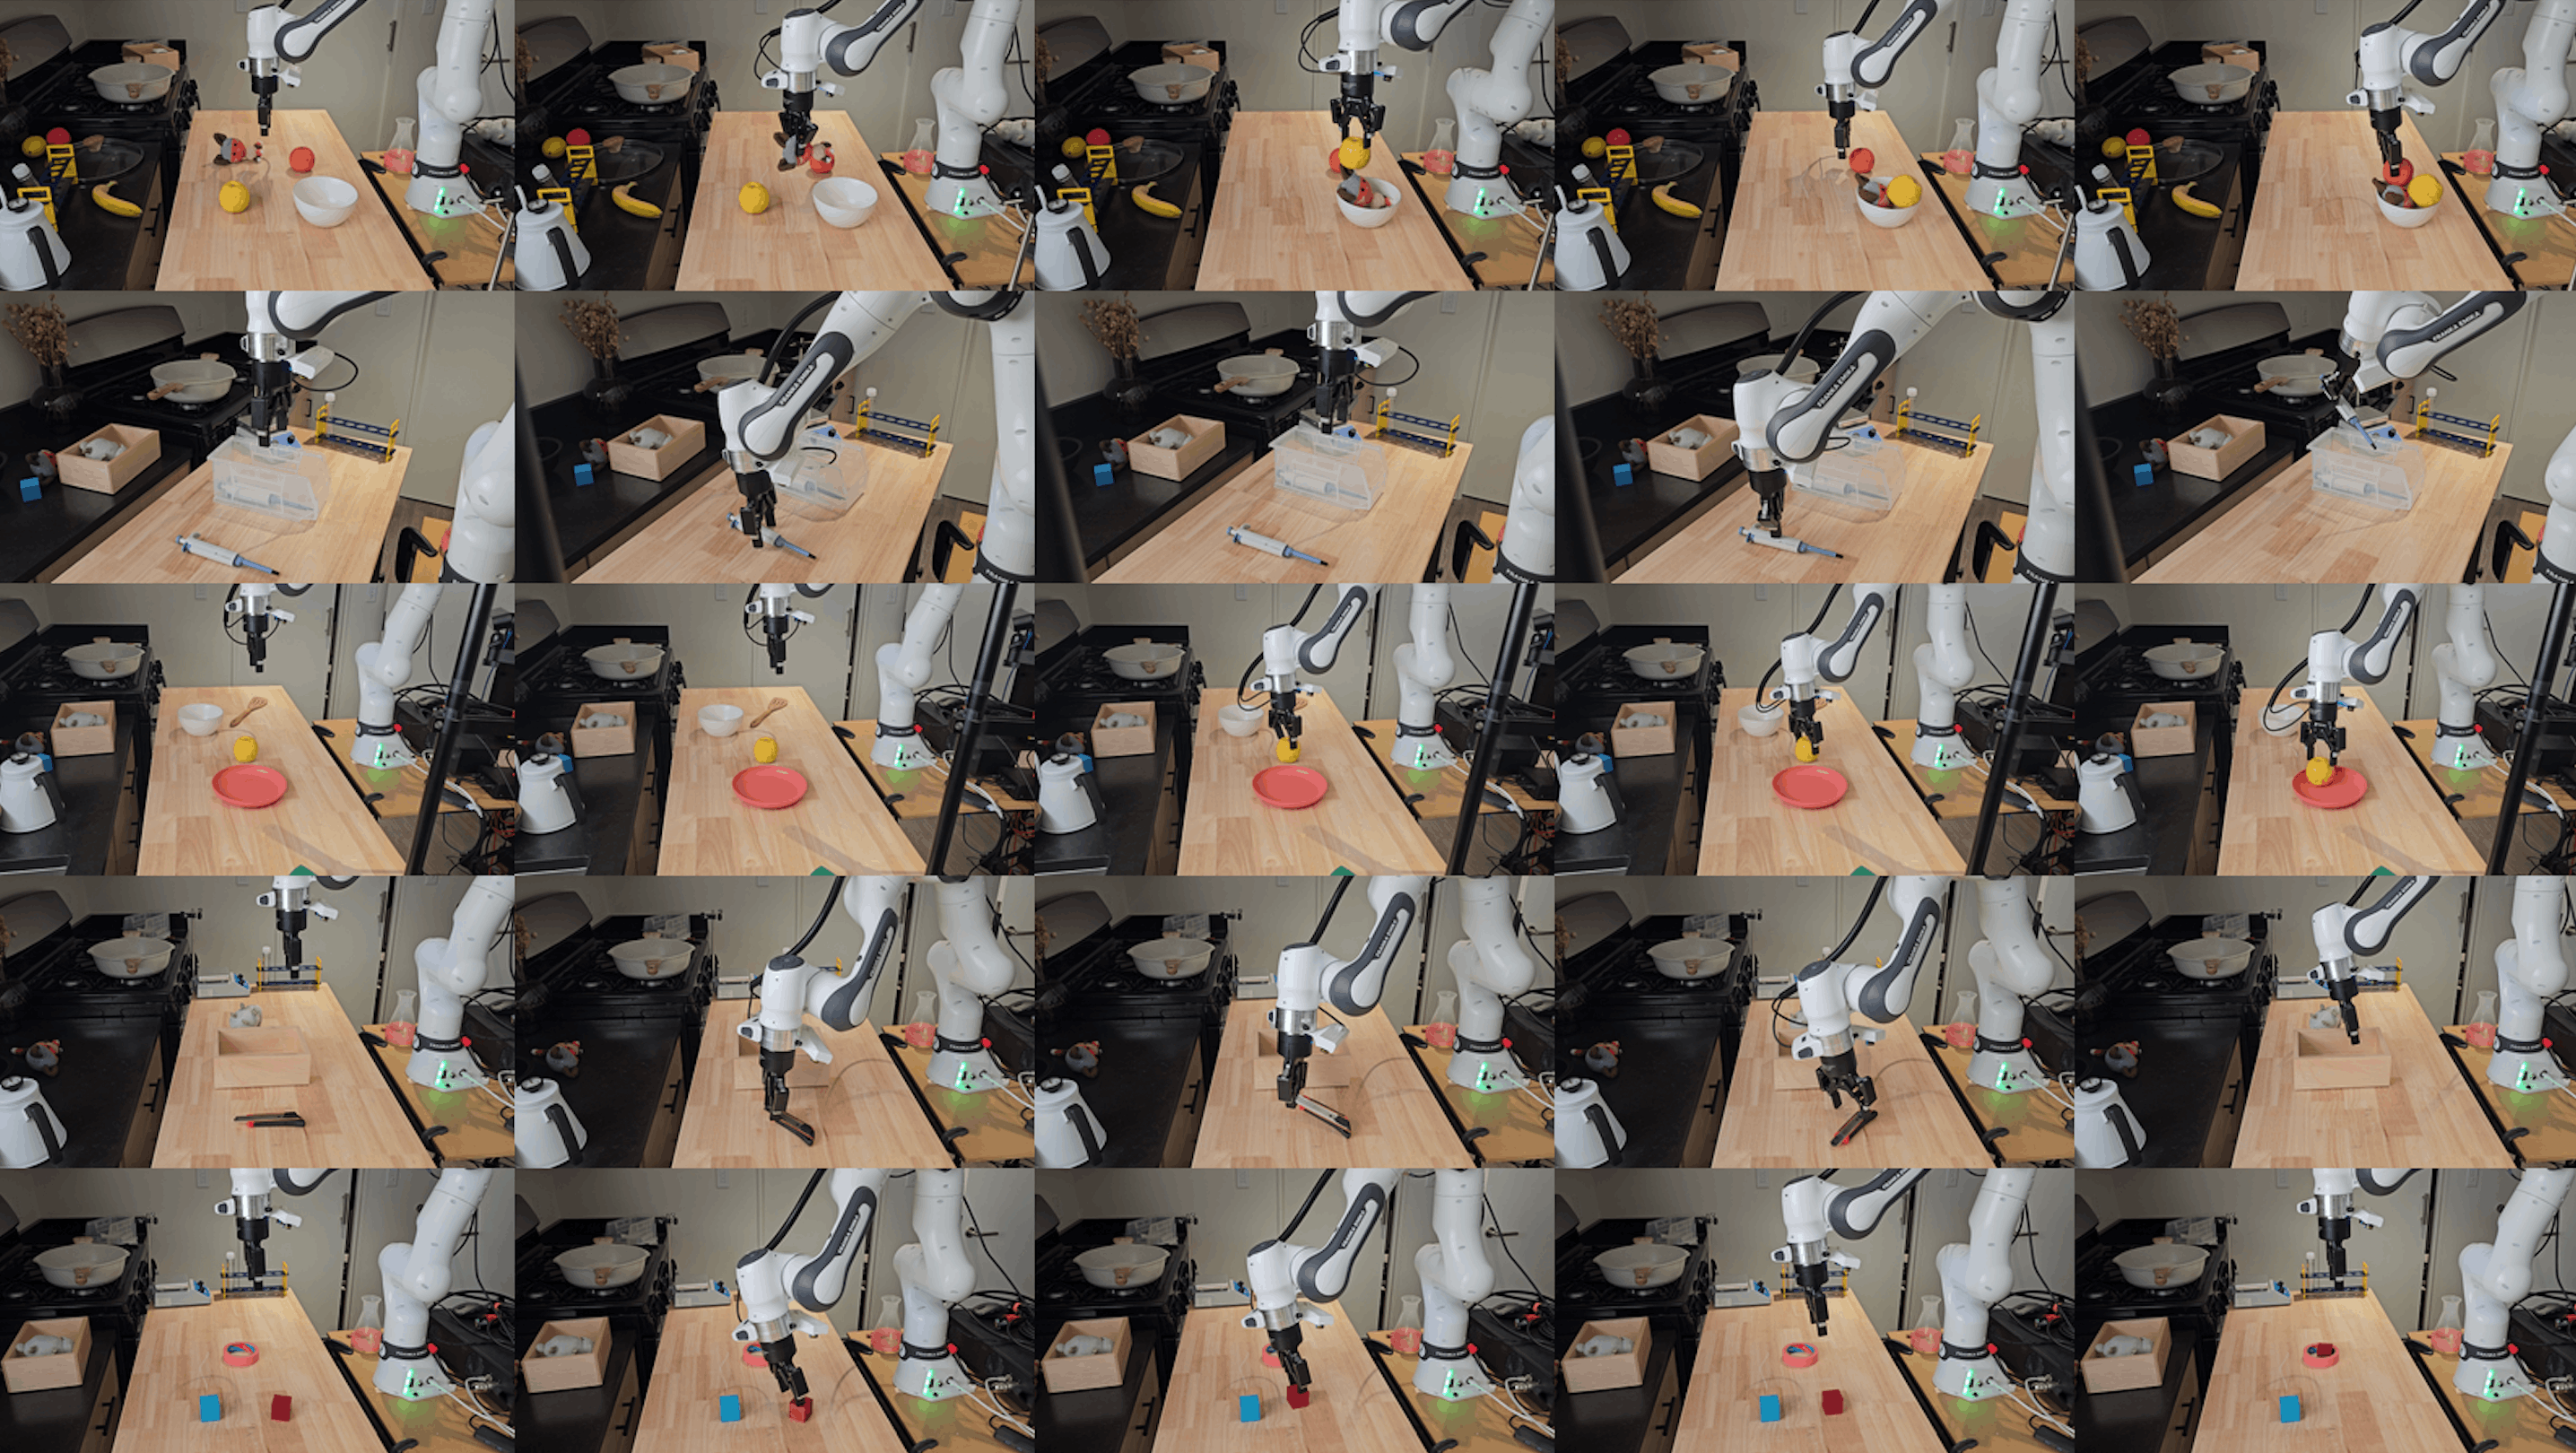
\includegraphics[width=\linewidth]{figures/s3.png}
    \caption{\textbf{Sample trajectories from the DROID evaluation of MolmoAct2.} }
    \label{fig:droid_sample}
\end{figure}


\begin{table}[h]
\centering
\caption{Per-task and per-position success rates across policies. Each task uses 15 trajectories (5 per position).}
\label{tab:policy-results}
\begin{threeparttable}
\begin{tabular}{llcccc}
\toprule
\textbf{Task} & \textbf{Policy} & \textbf{Pos.\ 1} & \textbf{Pos.\ 2} & \textbf{Pos.\ 3} & \textbf{Overall} \\
\midrule
\multirow{3}{*}{Put the apple on the plate}
  & MolmoAct2 & 5/5 (100\%) & 5/5 (100\%) & 5/5 (100\%) & \textbf{15/15 (100.0\%)} \\
  & $\pi_05$-DROID   & 5/5 (100\%) & 3/5 (60\%)  & 2/5 (40\%)  & 10/15 (66.7\%) \\
  & MolmoBot  & 5/5 (100\%) & 4/5 (80\%)  & 4/5 (80\%)  & 13/15 (86.7\%) \\
\midrule
\multirow{3}{*}{Put the pipette in the tray}
  & MolmoAct2 & 4/5 (80\%)  & 4/5 (80\%)  & 5/5 (100\%) & \textbf{13/15 (86.7\%)} \\
  & $\pi_05$-DROID   & 2/5 (40\%)  & 3/5 (60\%)  & 0/5 (0\%)   & 5/15 (33.3\%) \\
  & MolmoBot  & 3/5 (60\%)  & 2/5 (40\%)  & 3/5 (60\%)  & 8/15 (53.3\%) \\
\midrule
\multirow{3}{*}{Put the red cube inside the tape roll}
  & MolmoAct2 & 5/5 (100\%) & 4/5 (80\%)  & 5/5 (100\%) & \textbf{14/15 (93.3\%)} \\
  & $\pi_05$-DROID   & 3/5 (60\%)  & 5/5 (100\%) & 0/5 (0\%)   & 8/15 (53.3\%) \\
  & MolmoBot  & 1/5 (20\%)  & 0/5 (0\%)   & 4/5 (80\%)  & 5/15 (33.3\%) \\
\midrule
\multirow{3}{*}{Put the knife in the box}
  & MolmoAct2 & 5/5 (100\%) & 5/5 (100\%) & 4/5 (80\%)  & \textbf{14/15 (93.3\%)} \\
  & $\pi_05$-DROID   & 3/5 (60\%)  & 1/5 (20\%)  & 0/5 (0\%)   & 4/15 (26.7\%) \\
  & MolmoBot  & 1/5 (20\%)  & 0/5 (0\%)   & 5/5 (100\%) & 6/15 (40.0\%) \\
\midrule
\multirow{3}{*}{Put the objects in the bowl\tnote{a}}
  & MolmoAct2 & 73.2\% & 53.0\% & 59.8\% & \textbf{62.0\%} \\
  & $\pi_05$-DROID   & 39.6\% & 39.6\% & 59.4\% & 46.2\% \\
  & MolmoBot  & 33.0\% & 26.4\% & 26.4\% & 28.6\% \\
\bottomrule
\end{tabular}
\begin{tablenotes}\footnotesize
\item[a] Partial-credit task scored on $\{0,\,0.33,\,0.66,\,1.0\}$ per trajectory; reported as mean success rate.
\end{tablenotes}
\end{threeparttable}
\end{table}

\subsection{Real-world Bimanual YAM}
\textbf{Implementation.} We trained \molmoacttpos as eight separate single-task policies; to ensure a fair comparison, we applied the identical training protocol to each of the four baseline policies. All policies were trained to convergence, and the resulting checkpoints were used for evaluation. Evaluation and setup were carried out by Cortex AI: each task was collected under three spatial variants and evaluated under the same three variants.

\begin{figure}[htb!]
    \centering
    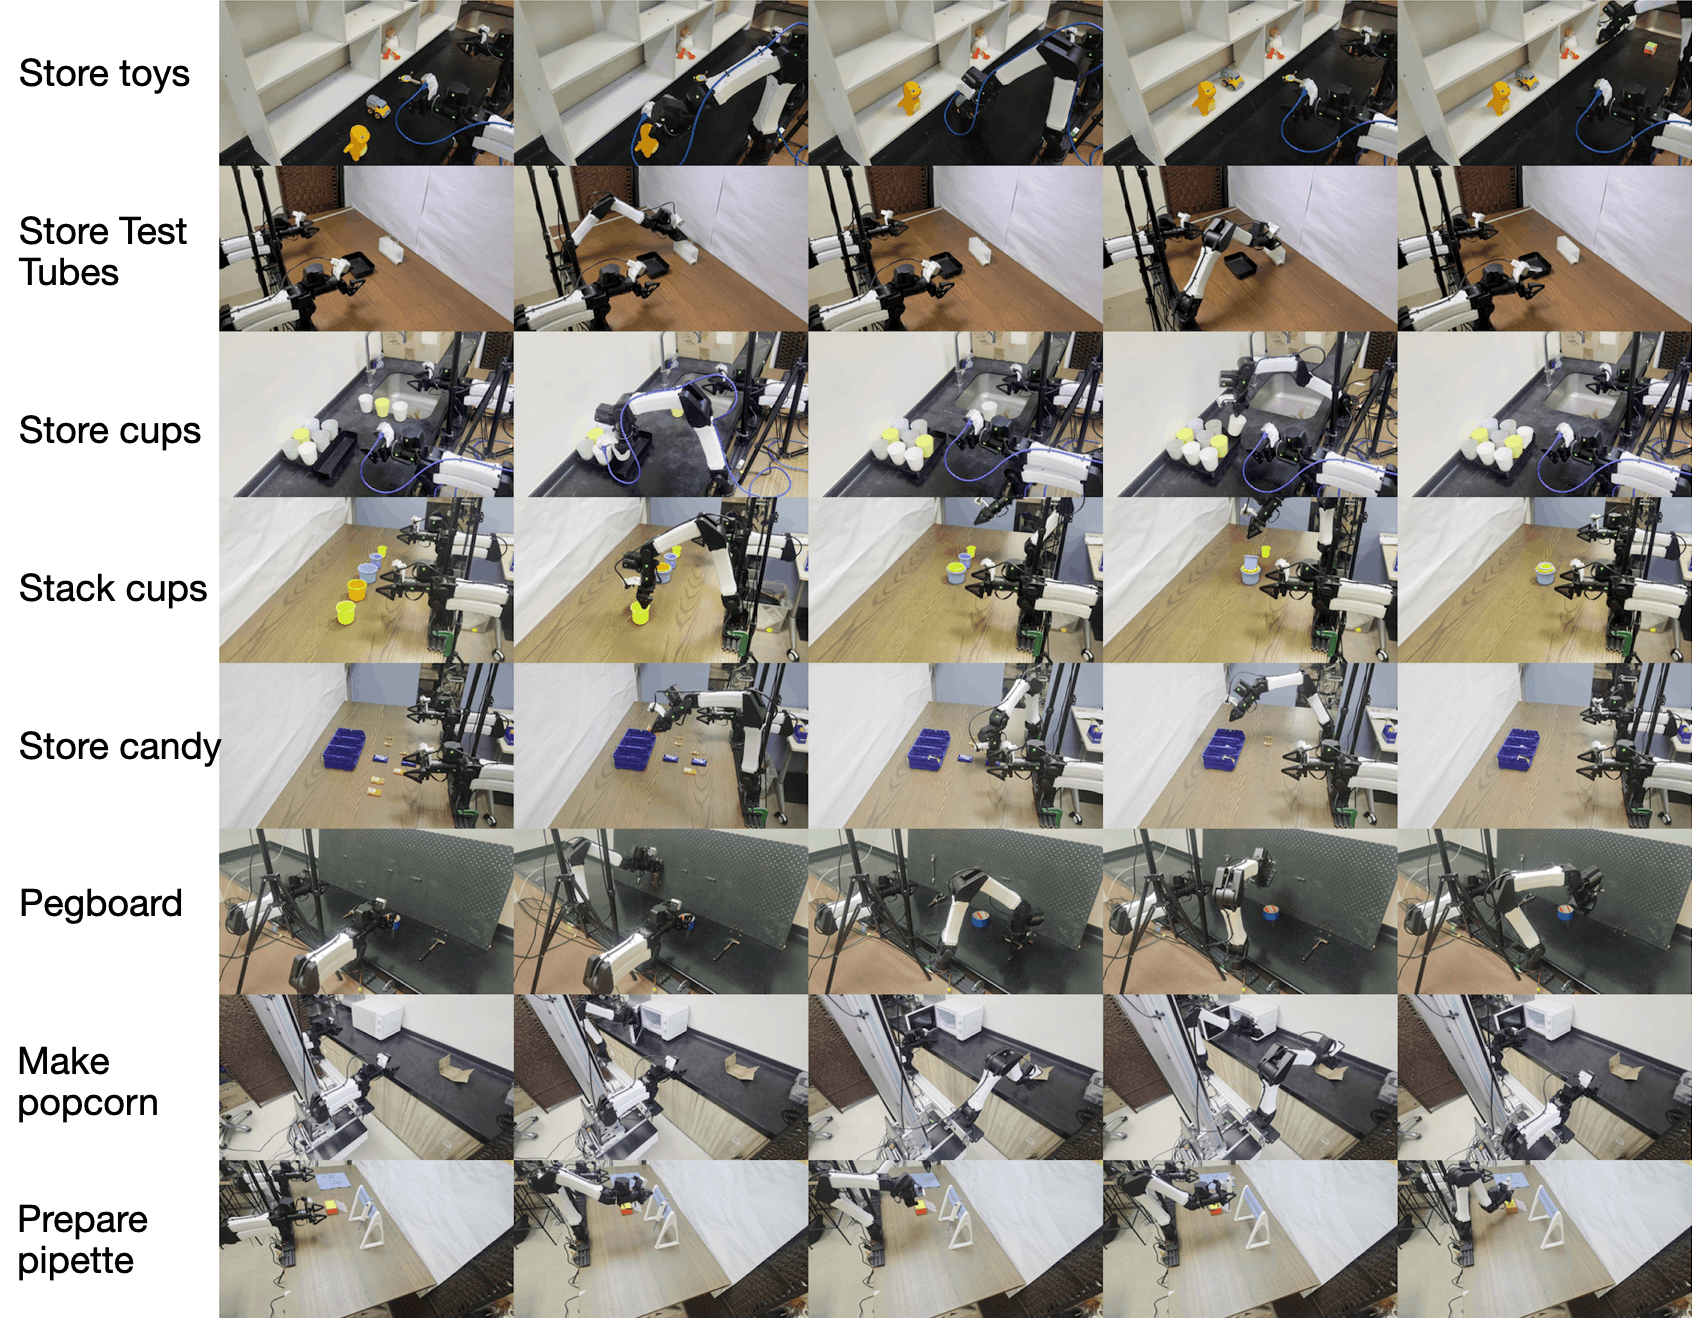
\includegraphics[width=\linewidth]{figures/s2.png}
    \caption{\textbf{Sample trajectories from the Bimanual YAM evaluation of MolmoAct2.} }
    \label{fig:so100_sample}
\end{figure}


\begin{figure}[htb!]
    \centering
    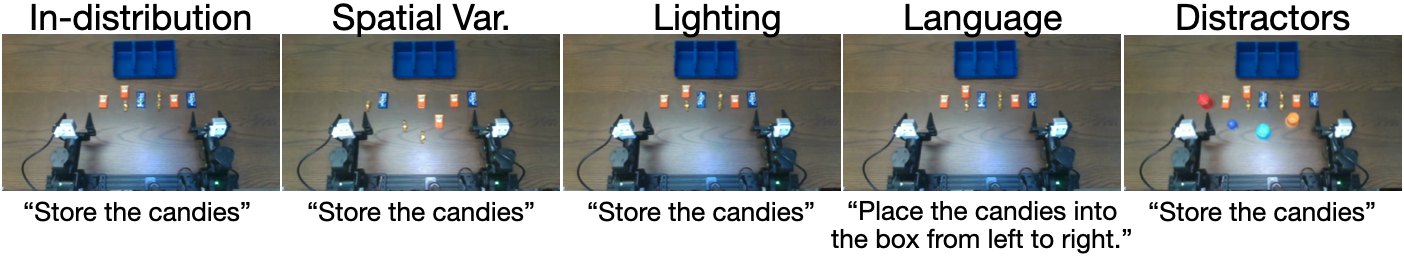
\includegraphics[width=\linewidth]{figures/ood.png}
    \caption{\textbf{Sample trajectories from the out-of-distribution Bimanual YAM evaluation of MolmoAct2.} }
    \label{fig:so100_sample}
\end{figure}


\begin{table}[t]
\centering
\caption{Overall success rate (\%) across 8 manipulation tasks (50 episodes each). Best model per task is \textbf{bold}.}
\label{tab:overall_results}
\setlength{\tabcolsep}{5pt}
\renewcommand{\arraystretch}{1.15}
\begin{tabular}{lccccc}
\toprule
\textbf{Task} & \textbf{$\pi_{0.5}$} & \textbf{Cosmos} & \textbf{X-VLA} & \textbf{OpenVLA} & \textbf{MolmoAct} \\
\midrule
Cup Stacking         & 62.0 & \textbf{64.5} & 5.5  & 60.5 & 54.0 \\
Linearbot            & 11.6 & 9.2  & 5.2  & 24.4 & \textbf{64.0} \\
Pegboard             & 2.0  & 0.0  & 3.0  & 4.5  & \textbf{14.0} \\
Cup Storing          & 85.9 & 0.0  & 7.9  & 96.0 & \textbf{100.0} \\
Candy Storing        & 26.0 & 0.0  & 3.8  & 26.5 & \textbf{40.5} \\
Store Test Tube      & 17.0 & 11.0 & 0.0  & 42.0 & \textbf{67.0} \\
Store Toys           & 26.0 & 7.0  & 2.5  & 2.0  & \textbf{32.0} \\
Prepare Pipette      & 27.5 & 32.0 & 11.5 & 28.5 & \textbf{33.0} \\
\midrule
\textbf{Average}     & 32.2 & 15.5 & 4.9  & 35.5 & \textbf{50.6} \\
\bottomrule
\end{tabular}
\end{table}

\subsection{Real-world SO-100/101 zero-shot}

\textbf{Implementation.} We conduct zero-shot evaluation on the SO-100 platform using a fixed, pre-initialized camera viewpoint, and compare against DePi and SmolVLA. Episodes are graded under a partial-credit scoring scheme, and no additional training of the policies is performed.

\begin{table*}[t]
\centering
\caption{Zero-shot success rate (\%) on SO-100 tasks with fixed initial camera position. Each task is graded with partial credit at three milestones; partial scores of 0.25, 0.5, and 1.0 are awarded for reaching the corresponding stage. 15 episodes per task. Best model per task is \textbf{bold}.}
\label{tab:so100_results}
\setlength{\tabcolsep}{5pt}
\renewcommand{\arraystretch}{1.2}
\begin{tabular}{lcccccc}
\toprule
& \multicolumn{3}{c}{\textbf{Partial-Credit Milestones}} & \multicolumn{3}{c}{\textbf{Success Rate (\%)}} \\
\cmidrule(lr){2-4}\cmidrule(lr){5-7}
\textbf{Task} & \textbf{0.25} & \textbf{0.5} & \textbf{1.0} & \textbf{SmolVLA} & \textbf{MolmoAct v2} & \textbf{DePi$_0$} \\
\midrule
Place fork on plate     & reach & pickup fork  & place on plate & 3.3 & \textbf{70.0} & 30.0          \\
Stack blocks            & reach & pickup block & stack blocks   & 5.0 & \textbf{20.0} & 6.7           \\
Place tissues in basket & reach & pickup       & place          & 0.0 & \textbf{73.3} & 20.0          \\
Place pen on notebook   & reach & pickup       & place          & 3.3 & \textbf{86.7} & 80.0          \\
Place block in box      & reach & pickup       & place          & 0.0 & 33.3          & \textbf{90.0} \\
\midrule
\multicolumn{4}{l}{\textbf{Average}} & 2.3 & \textbf{56.7} & 45.3 \\
\bottomrule
\end{tabular}
\end{table*}



\begin{figure}[htb!]
    \centering
    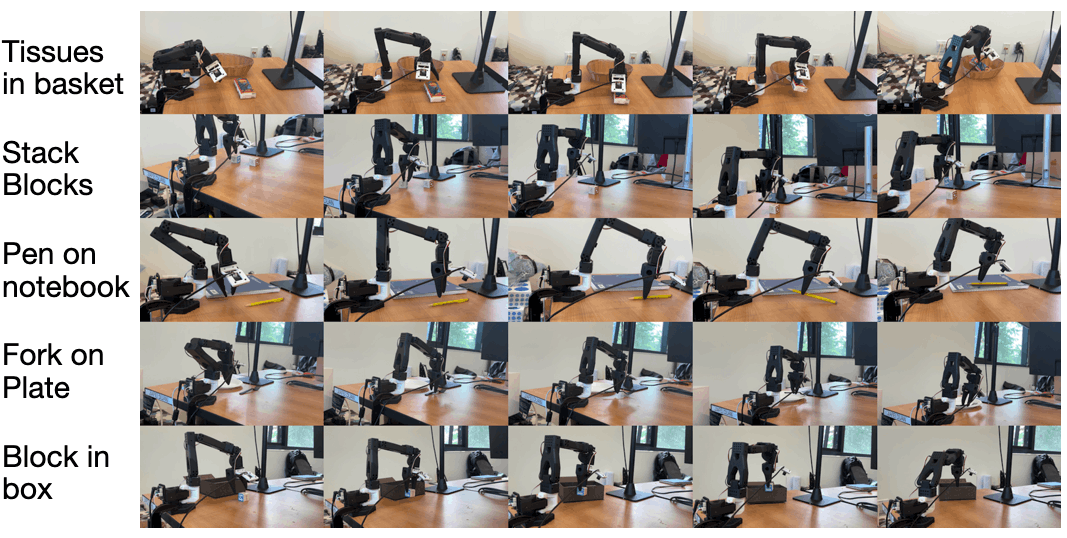
\includegraphics[width=\linewidth]{figures/s1.png}
    \caption{\textbf{Sample trajectories from the SO-100 evaluation of MolmoAct2.} }
    \label{fig:so100_sample}
\end{figure}

\clearpage

\section{Data Details}
\label{supp:data}
\subsection{\molmoacttsodata Statistics}
\label{supp:so100-so101-stats}

We use \molmoacttsodata in the \molmoactt training mixture. We first collect 1{,}660 dataset entries; then we use TOPReward \citep{chen2026topreward} to filter out 438
low-quality dataset entries, yielding 1{,}222 final
datasets. All statistics below are computed only over this final filtered set. \Cref{tab:so100-so101-summary} presents the summary statistics for the SO-100/101 training partition. \Cref{tab:so100-so101-robot-type} presents the number of datasets by the type of SO-10x variants. \Cref{tab:so100-so101-metadata} presents the distribution of different metadata such as FPS, camera configuration, and action/state dimensions. \Cref{fig:action_verbs} presents the distribution of action verbs before and after the language annotation pipeline described in \Cref{sec:lang_annot}. \Cref{fig:so100_sample} shows several sample trajectories from the dataset partition. 
\begin{figure}[htb!]
    \centering
    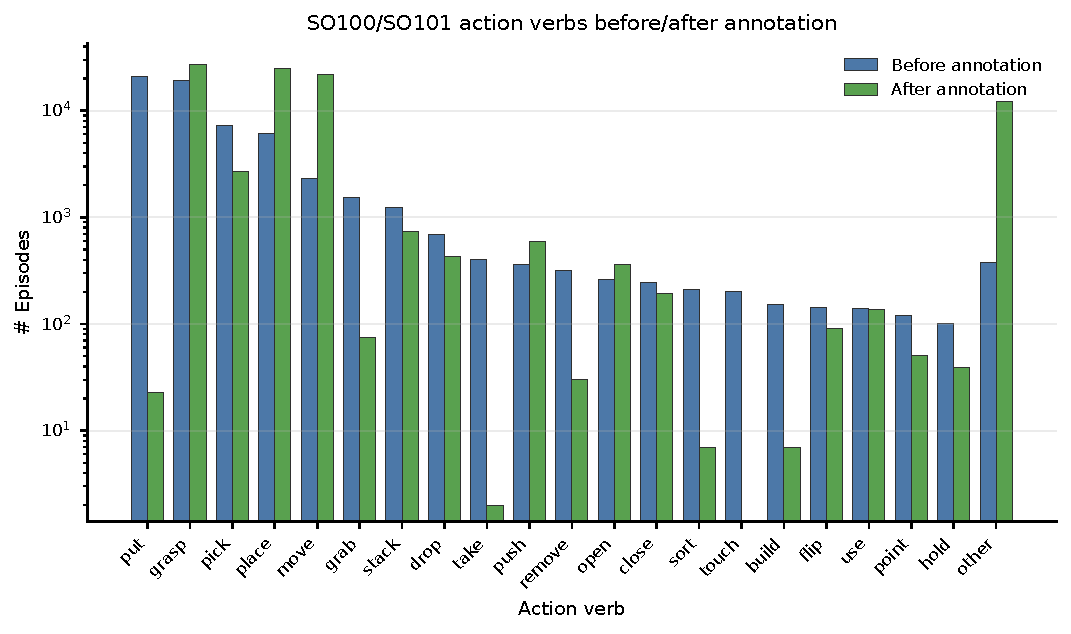
\includegraphics[width=0.9\linewidth]{figures/so100_annotation_before_after_action_verb_histogram.pdf}
    \caption{\textbf{Action verb distribution before and after language annotation.} }
    \label{fig:action_verbs}
\end{figure}

\begin{figure}[htb!]
    \centering
    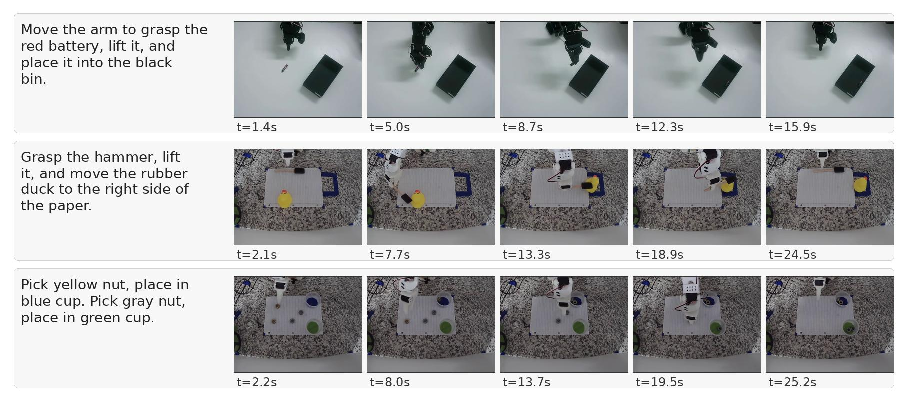
\includegraphics[width=0.9\linewidth]{figures/so100_sample_episode_frames.pdf}
    \caption{\textbf{Sample trajectories from the SO10x dataset partition.} }
    \label{fig:so100_sample}
\end{figure}


\begin{table}[ht]
\centering
\footnotesize
\caption{\textbf{Summary statistics for the SO-100/101 training subset.} We
report statistics for the final filtered \molmoacttsodata partition.}
\setlength{\tabcolsep}{6pt}
\renewcommand{\arraystretch}{1.1}
\begin{tabular}{lr}
% \toprule
\textbf{Statistic} & \textbf{Value} \\
\midrule
\# datasets & 1{,}222 \\
Contributors & 377 \\
Episodes & 38{,}059 \\
Frames & 19.8M \\
Estimated duration & 183.6 hours \\
Metadata task count & 1{,}322 \\
Instruction rows & 38{,}059 \\
Globally unique instructions & 12{,}818 \\
Unique-instruction ratio & 33.7\% \\
Datasets with annotated task metadata & 1{,}222 \\
% \bottomrule
\end{tabular}
\label{tab:so100-so101-summary}
\end{table}

\begin{table}[t]
\centering
\footnotesize
\caption{\textbf{SO-10x data partition breakdown by robot type.}}
\setlength{\tabcolsep}{5pt}
\renewcommand{\arraystretch}{1.1}
\begin{tabular}{lrrrr}
% \toprule
\textbf{Robot type} & \textbf{Datasets} & \textbf{Episodes} & \textbf{Frames} & \textbf{Hours} \\
\midrule
SO-100 & 921 & 31{,}101 & 15.18M & 141.7 \\
SO-101 & 299 & 6{,}898 & 4.57M & 41.6 \\
MOSS & 2 & 60 & 15.6K & 0.2 \\
% \bottomrule
\end{tabular}
\label{tab:so100-so101-robot-type}
\end{table}



\begin{table}[t]
\centering
\footnotesize
\caption{\textbf{Recording and feature metadata.} Most demonstrations are
recorded at 30 Hz with two camera streams; all final filtered datasets use
six-dimensional action and state vectors.}
\setlength{\tabcolsep}{6pt}
\renewcommand{\arraystretch}{1.1}
\begin{tabular}{lrrrr}
% \toprule
\textbf{Metadata field} & \textbf{Value} & \textbf{Datasets} & \textbf{Episodes} & \textbf{Frames} \\
\midrule
FPS & 30 & 1{,}114 & 36{,}828 & 18.96M \\
FPS & 20 & 78 & 527 & 261.4K \\
FPS & 25 & 18 & 423 & 256.7K \\
FPS & 60 & 8 & 208 & 231.6K \\
Camera count & 1 & 230 & 4{,}159 & 2.26M \\
Camera count & 2 & 835 & 24{,}151 & 13.05M \\
Camera count & 3 & 151 & 9{,}235 & 4.11M \\
Camera count & 4 & 6 & 514 & 342.1K \\
Action dimension & 6 & 1{,}222 & 38{,}059 & 19.76M \\
State dimension & 6 & 1{,}222 & 38{,}059 & 19.76M \\
% \bottomrule
\end{tabular}
\label{tab:so100-so101-metadata}
\end{table}

\subsection{Language Annotation Pipeline Implementation Details}
\label{supp:language-annotation-details}
Running inference with temperature 0.1 and max\_length set to 1024 tokens, we feed the following prompt into Qwen3.5-27B:
\begin{quote} 
You are an expert robot arm task instruction generator. You are provided with multiple demonstration videos, each showing the exact same task execution captured simultaneously from different camera angles. The task is to \{original\_instruction\}. Based on these videos, generate a clear imperative instruction describing all of the actions performed by the robot arm. Carefully study the evolution of the state of the scene, to understand how the robot arm achieves the goal. Pay attention to the color and position of the objects the robot interacts with. Start directly with an action verb and make sure you do not miss any actions. Note that the robot arm is not always grasping an object and maybe pushing objects around instead. Verify any grasps by checking the gripper state, and only say the arm is grasping an object if this is shown in the wrist camera when the gripper is closed. Your prompts should be almost exactly \{word\_limit\} words long.
\end{quote}

 word\_limit is a number randomly sampled from a right tailed power distribution, with a minimum value of 5 and a maximum value of 25. In addition to the text prompt, for each of the cameras in the trajectory that are not frozen, we sample 12 frames that are each equally temporally spaced and pass the frames to the model. 
 
 Running this pipeline results in the changes to the number of unique instructions in the datasets shown in Table \ref{tab:language-annot_increased}.

\begin{table}[t]
\centering
\footnotesize
\caption{\textbf{Dataset Language Annotation Diversity.} Running the language annotation pipeline increases the number of unique instructions for all of the robotics datasets in \molmoactt's training mix.}
\setlength{\tabcolsep}{5pt}
\renewcommand{\arraystretch}{1.1}
\begin{tabular}{lcc}
% \toprule
\textbf{Dataset} & \textbf{Original Instructions} & \textbf{Relabeled Instructions}\\
\midrule
\molmoacttyamdata & 34 (0.1\%)     & 11448 (35\%)   \\
\midrule
\molmoacttdroiddata            & 49623 (67\%)   & 55905 (75\%)   \\
\midrule
\molmoacttsodata            & 707 (1.5\%)    & 16205 (34\%)   \\
\midrule
\molmoactdata       & 134 (1\%)      & 2959 (28\%)    \\
\midrule
BC-Z             & 104 (0.3\%)    & 9981 (25\%)    \\
\midrule
Fractal          & 598 (0.7\%)    & 16729 (19\%)   \\
\midrule
Bridge           & 19973 (37\%)   & 35096 (66\%)   \\
\midrule
\textbf{Total}   & \textbf{71121 (22\%)} & \textbf{146485 (46\%)} \\
\end{tabular}
\label{tab:language-annot_increased}
\end{table}


% \subsection{Past tabletop bimanual manipulation datasets}
\begin{table}[t]
\centering
\footnotesize
\caption{\textbf{Past Tabletop Bimanual Manipulation Datasets.} \molmoacttyamdata is the largest open-source tabletop bimanual robotics dataset. In this table, we compare against other open and closed-source tabletop bimanual datasets from the literature.}
\setlength{\tabcolsep}{5pt}
\renewcommand{\arraystretch}{1.1}
\begin{tabular}{lccc}
\toprule
\textbf{Dataset Name} & \textbf{Embodiment} & \textbf{Number of Trajectories} & \textbf{Open / Closed?}\\
\midrule
{\color{ai2pink}\molmoacttyamdata (Ours)} & {\color{ai2pink}Bimanual YAM} & {\color{ai2pink}34,500} & {\color{ai2pink}Open}  \\ 
\midrule
AIST Bimanual Manipulation Dataset~\citep{motoda2025aistdata} & ALOHA & 10,000 & Open \\ 
\midrule
BiPlay Dataset~\citep{dasari2025ingredients} & ALOHA & 7,000 & Open \\ 
\midrule
RDT-1B Finetuning Dataset~\citep{liu2024rdt} & ALOHA & 6,000 & Open \\ 
\midrule
ALOHA Unleashed Training Data~\citep{zhao2024aloha} & ALOHA & 26,000 & Closed \\
\midrule
SARM RA-BC Dataset~\citep{chen2025sarm} & Bimanual YAM & 200 Hours & Closed \\ 
\bottomrule
\end{tabular}
\label{tab:past_robot_data}
\end{table}

% \begin{table}[t]
% \centering
% \footnotesize
% \caption{\textbf{Previous  open-source robotics manipulation datasets} TODO}
% \setlength{\tabcolsep}{5pt}
% \renewcommand{\arraystretch}{1.1}
% \begin{tabular}{l p{0.3\linewidth} c}
% % \toprule
% \textbf{Dataset Name} & \textbf{Embodiment} & \textbf{Number of Trajectories}\\
% \midrule
% AGIBot World~\citep{agibotworldcontributors2025agibotworldcolosseolargescale} & AGIBot & 1,000,000 \\ 
% \midrule
% RoboMIND 2.0~\citep{hou2025robomind} & Franka, Ur5E, AgileX, ARX, TienKung, TianYi & 310,000 \\ 
% \midrule
% RoboNet~\citep{dasari2019robonet} & Franka, WidowX, Sawyer, Baxter, Kuka, Fetch, Google Robot & 162,000 \\
% \midrule
% RH20T~\citep{fang2023rh20t} & Franka, Kuka, UR5, Flexiv & 110,000 \\
% \midrule
% Galaxea Open-World Dataset~\citep{jiang2025galaxea} & Galaxea R1 Lite & 100,000 \\ 
% % \bottomrule
% \end{tabular}
% \label{tab:past_robot_data}
% \end{table}
% \subsection{Action Reasoning Data}

% We construct the \emph{Action Reasoning Data} by converting conventional robot episodes $(I_t, L, A_t)$ into an augmented autoregressive sequence in which each timestep is supplemented with two additional supervisory signals: discretized depth tokens and a visual reasoning trace. Depth targets are obtained by inferring dense depth maps from RGB observations using DepthAnything-v2, followed by quantization with a VQ-VAE trained for 20~epochs on 10~million tabletop manipulation images, yielding an $h \times w$ grid of codebook indices that serve as the \textsc{DepthTokens}. The visual reasoning trace consists of a sequence of pixel coordinates representing the projected near-future motion of the end-effector, obtained by prompting a vision–language model to localize the gripper in each frame and selecting one to five points spanning from the current timestep to a designated future index. The resulting sequence for each timestep comprises the depth tokens, the visual reasoning trace, and the action vector (end-effector pose delta and gripper state), which are used jointly for autoregressive training with cross-entropy over discrete tokens and an $\ell_1$ loss over continuous action parameters. The final corpus contains 21{,}101{,}636 labeled frames, sourced from \textsc{BC-Z} (10{,}289{,}224; 48.8\%), \textsc{RT-1} (7{,}065{,}620; 33.5\%), and \textsc{Bridge-v2} (3{,}746{,}792; 17.8\%). Unless otherwise specified, mini-batches are sampled in proportion to these dataset shares to maintain source distribution during training. We defined the task, its description, the corresponding language instruction, and the task progression metric ratings.

% Ascii







% \subsection{\molmoactdata}

% \molmoactdata has two external camera views and a single wrist camera view. In the home environment data, the camera view configuration may vary between tasks, whereas for the tabletop data it remains the same for all tasks. For each task, we first rank the two external camera views based on scene clarity (i.e., how well the robot and objects are visible) and whether the view is occluded by the robot during task execution. Based on this ranking, we label them as the \textit{primary} and \textit{secondary} camera views. All home environment data is recorded at 15 Hz, while all tabletop data is recorded at 20 Hz. The tabletop data additionally includes extrinsic and intrinsic camera calibration matrices for both external cameras available on . We list details of the tasks we collected for \molmoact Dataset in Table \ref{tab:home_task} and \ref{tab:tabletop_task}. 


      
% \begin{table}[t]
% \centering
% \begingroup
% \setlength{\tabcolsep}{1pt}
% \setlength{\arrayrulewidth}{0.1pt}
% \renewcommand{\arraystretch}{1.1}
% \scriptsize
% \begin{tabular}{|p{0.11\linewidth}|p{0.26\linewidth}|p{0.34\linewidth}|p{0.25\linewidth}|}
% \hline
% \textbf{Scene} & \textbf{Task} & \textbf{Language Instruction} & \textbf{Object(s)} \\
% \hline
% \csvreader[
%   separator=comma,
%   head to column names,
%   late after line=\\\hline
% ]{\detokenize{tables/appendix/MolmoAct_Dataset_home.csv}}{}%
% {\csvcoliii & \texttt{\csvcoli} & \csvcolii & \csvcoliv}
% \end{tabular}
% \caption{Tasks details of \molmoactdata Home Environemnt including scene, task name, language instruction and all objects used for data collection.}
% \label{tab:home_task}
% \endgroup
% \end{table}



% \begin{table}[t]
% \centering
% \begingroup
% \setlength{\tabcolsep}{1pt}
% \setlength{\arrayrulewidth}{0.1pt}
% \renewcommand{\arraystretch}{1.1}
% \scriptsize
% \begin{tabular}{|p{0.11\linewidth}|p{0.26\linewidth}|p{0.34\linewidth}|p{0.25\linewidth}|}
% \hline
% \textbf{Scene} & \textbf{Task} & \textbf{Language Instruction} & \textbf{Object(s)} \\
% \hline
% \csvreader[
%   separator=comma,
%   head to column names,
%   late after line=\\\hline
% ]{\detokenize{tables/appendix/MolmoAct_Dataset_tabletop.csv}}{}%
% {\csvcoliii & \texttt{\csvcoli} & \csvcolii & \csvcoliv}
% \end{tabular}
% \caption{Tasks details of \molmoactdata Tabletop Environemnt including scene, task name, language instruction and all objects used for data collection.}
% \label{tab:tabletop_task}
% \endgroup
% \end{table}



% \begin{table}[t]
% \centering
% \begingroup
% \setlength{\tabcolsep}{2pt}        % was 4pt; tighter padding, same column widths
% \setlength{\arrayrulewidth}{0.3pt} % slightly thinner vertical lines
% \renewcommand{\arraystretch}{1.1}
% \scriptsize
% \begin{tabular}{|p{0.08\linewidth}|p{0.26\linewidth}|p{0.34\linewidth}|p{0.28\linewidth}|}
% \hline
% \textbf{Scene} & \textbf{Task} & \textbf{Language Instruction} & \textbf{Object(s)} \\
% \hline
% \csvreader[
%   separator=comma,
%   head to column names,
%   late after line=\\\hline
% ]{figures/Molmo-ACT_Dataset.csv}{}%
% {\csvcoliii & \texttt{\csvcoli} & \csvcolii & \csvcoliv}
% \end{tabular}
% \caption{Prompts from \texttt{figures/Molmo-ACT_Dataset.csv} grouped by scene order.}
% \label{tab:molmoact_task_detail}
% \endgroup
% \end{table}

\clearpage

% \section{Data Examples}
\label{supp:dataexamples}


This section include \textbf{randomly selected} examples from \molmoact's Action Reasoning Data and Multimodal web data used in pre-training, as well as \molmoactdata used in mid-training, and demonstrations collected for post-training. Prompts are shown in bold and Visual Reasoning Trace are annotated with a yellow line.

\begin{itemize}
    \item \textbf{Action Reasoning Data - Figure \ref{fig:appendix_action_reasoning_data_1}}
    \item \textbf{Auxiliary Visual Reasoning Trace - Figure \ref{fig:appendix_line} }
    \item \textbf{Auxiliary Depth Perception Tokens - Figure \ref{fig:appendix_depth}}
    \item \textbf{Trajectory-conditioned Action Data - Figure \ref{fig:appendix_trajectory}}
    \item \textbf{Multimodal Web Data - Figure \ref{fig:appendix_vqa}}
    \item \textbf{\molmoactdata (Home Environment) - Figure \ref{fig:appendix_molmoactdataset_home}}
    \item \textbf{\molmoactdata (Tabletop) - Figure \ref{fig:appendix_molmoactdataset_tabletop}}
    \item \textbf{Post-Training Single Arm Franka - Figure \ref{fig:appendix_singlearm}}
    \item \textbf{Post-Training Bimanual Franka - Figure \ref{fig:appendix_bimanual}}
    \item \textbf{Post-Training Rainbow - Figure \ref{fig:appendix_rainbow}}
    
\end{itemize}



\begin{figure*}[t]  
  \centering
  \includegraphics[width=\textwidth]{figures/Appendix/Data_Examples/Appendix_Action_Reasoning_1.pdf}
  \caption{Randomly selected examples from \textbf{Action Reasoning Data} used in the pre-training stage.}

  \label{fig:appendix_action_reasoning_data_1}
\end{figure*}



\begin{figure*}[t]  
  \centering
  \includegraphics[width=\textwidth]{figures/Appendix/Data_Examples/Appendix_Line_2.pdf}
  \caption{Randomly selected examples from \textbf{Auxiliary Visual Reasoning Trace} data used in the pre-training stage.}

  \label{fig:appendix_line}
\end{figure*}






\begin{figure*}[t]  
  \centering
  \includegraphics[width=\textwidth]{figures/Appendix/Data_Examples/Appendix_Depth_2.pdf}
  \caption{Randomly selected examples from \textbf{Auxiliary Depth Perception Tokens} data used in the pre-training stage.}

  \label{fig:appendix_depth}
\end{figure*}

\begin{figure*}[t]  
  \centering
  \includegraphics[width=\textwidth]{figures/Appendix/Data_Examples/Appendix_Trajectory.pdf}
  \caption{Randomly selected examples from \textbf{Trajectory-conditioned Action Data} used in the pre-training stage.}

  \label{fig:appendix_trajectory}
\end{figure*}



\begin{figure*}[t]  
  \centering
  \includegraphics[width=\textwidth]{figures/Appendix/Data_Examples/Appendix_VQA.pdf}
  \caption{Randomly selected examples from \textbf{Multimodal Web Data} used in the pre-training stage.}

  \label{fig:appendix_vqa}
\end{figure*}


\begin{figure*}[t]  
  \centering
  \includegraphics[width=\textwidth]{figures/Appendix/Data_Examples/Appendix_Molmoact_Home.pdf}
  \caption{Randomly selected examples from \textbf{\molmoactdata (Home Environment)} used in the mid-training stage.}

  \label{fig:appendix_molmoactdataset_home}
\end{figure*}



\begin{figure*}[t]  
  \centering
  \includegraphics[width=\textwidth]{figures/Appendix/Data_Examples/Appendix_Molmoact_Tabletop.pdf}
  \caption{Randomly selected examples from \textbf{\molmoactdata (Tabletop Environment)} used in the mid-training stage.}

  \label{fig:appendix_molmoactdataset_tabletop}
\end{figure*}


\begin{figure*}[t]  
  \centering
  \includegraphics[width=\textwidth]{figures/Appendix/Data_Examples/Appendix_SingleArm.pdf}
  \caption{Randomly selected examples from \textbf{Single Arm Franka} demonstrations used in the post-training stage.}

  \label{fig:appendix_singlearm}
\end{figure*}


\begin{figure*}[t]  
  \centering
  \includegraphics[width=\textwidth]{figures/Appendix/Data_Examples/Appendix_Bimanual.pdf}
  \caption{Randomly selected examples from \textbf{Bimanual Franka} demonstrations used in the post-training stage.}

  \label{fig:appendix_bimanual}
\end{figure*}




\begin{figure*}[t]  
  \centering
  \includegraphics[width=\textwidth]{figures/Appendix/Data_Examples/Appendix_Rainbow.pdf}
  \caption{Randomly selected examples from \textbf{Rainbow} demonstrations used in the post-training stage.}

  \label{fig:appendix_rainbow}
\end{figure*}

% % \clearpage

\section{Limitations and Potential Solutions}
\label{supp:limit}

While \molmoactt is all quite capable as a general-purpose action reasoning model, it is not without limitations. In the following sections, we discuss some of these limitations and potential solutions.

\paragraph{Action chunks and the absence of real-time re-chunking.}
\molmoactt predicts fixed-horizon action chunks (30 steps at 30~Hz for YAM/SO-100/101, 15 at 15~Hz for DROID, 10 at 10~Hz for LIBERO) and executes them open-loop before re-querying the policy. This has two consequences worth acknowledging. First, motion smoothness across chunk boundaries is not enforced anywhere in the pipeline: the flow-matching expert is trained to denoise each chunk independently, with no continuity loss tying the end of chunk $t$ to the start of chunk $t+1$. In practice this can produce visible velocity or acceleration discontinuities at the seams, particularly when the VLM context shifts between queries (new observation, slightly different attention state). Second, because the policy commits to a full chunk before observing its consequences, it cannot react within-chunk to perturbations, contact events, or its own tracking error --- the 55.79~Hz number in Sec \ref{speed} is amortized chunk throughput, not closed-loop reactivity.

\paragraph{Embodiment-specific zero-shot deployment.}
The zero-shot deployment story for \textsc{MolmoAct2} is currently tied to the three embodiments for which we have large-scale training data: \molmoacttyam, \molmoacttso, and \molmoacttdroid can each be deployed out-of-the-box on their respective robot setups (bimanual YAM, SO-100/101, and DROID Franka) Sec. \ref{sec:exp-outbox}. This is a direct consequence of our data strategy --- concentrating collection and curation effort on these three platforms to span the low-to-medium cost range --- but it also bounds what zero-shot means here. \textsc{MolmoAct2} is not a universal controller that transfers without adaptation to arbitrary new embodiments: deployment on robots outside this set (e.g., other bimanual platforms, dexterous hands, mobile manipulators with different kinematics, or humanoids) requires effective fine-tuning on target-embodiment demonstrations, as shown in our fine-tuning studies in Sec \ref{sec:exp-ft}. Extending the zero-shot envelope to a broader range of embodiments is a matter of scaling data collection along the same axes we have begun here, and we view the released datasets and training recipe as a foundation for that effort rather than a finished product.


